\documentclass{exam}

\usepackage[utf8]{inputenc}
\usepackage{array}
\usepackage{graphicx}
\usepackage{caption}
\usepackage{float}

%\newcolumntype{L}[1]{>{\raggedright\let\newline\\\arraybackslash\hspace{0pt}}m{#1}}
\usepackage{amsmath}

\newcounter{eqn}
\renewcommand*{\theeqn}{\alph{eqn})}
\newcommand{\num}{\refstepcounter{eqn}\text{\theeqn}\;}


\makeatletter
\newcommand{\putindeepbox}[2][0.7\baselineskip]{{%
    \setbox0=\hbox{#2}%
    \setbox0=\vbox{\noindent\hsize=\wd0\unhbox0}
    \@tempdima=\dp0
    \advance\@tempdima by \ht0
    \advance\@tempdima by -#1\relax
    \dp0=\@tempdima
    \ht0=#1\relax
    \box0
}}
\makeatother


\title{Questionary}

\begin{document}

\maketitle
%\section*{Questionary}

\section*{Frontend}

\subsection*{Color Theme}

The following images show different color themes of a table, containing patient information. 
Red rows indicate that our algorithm detected a potential decubitus risk. 

\begin{tabular}{cc}
	\num\putindeepbox[7pt]{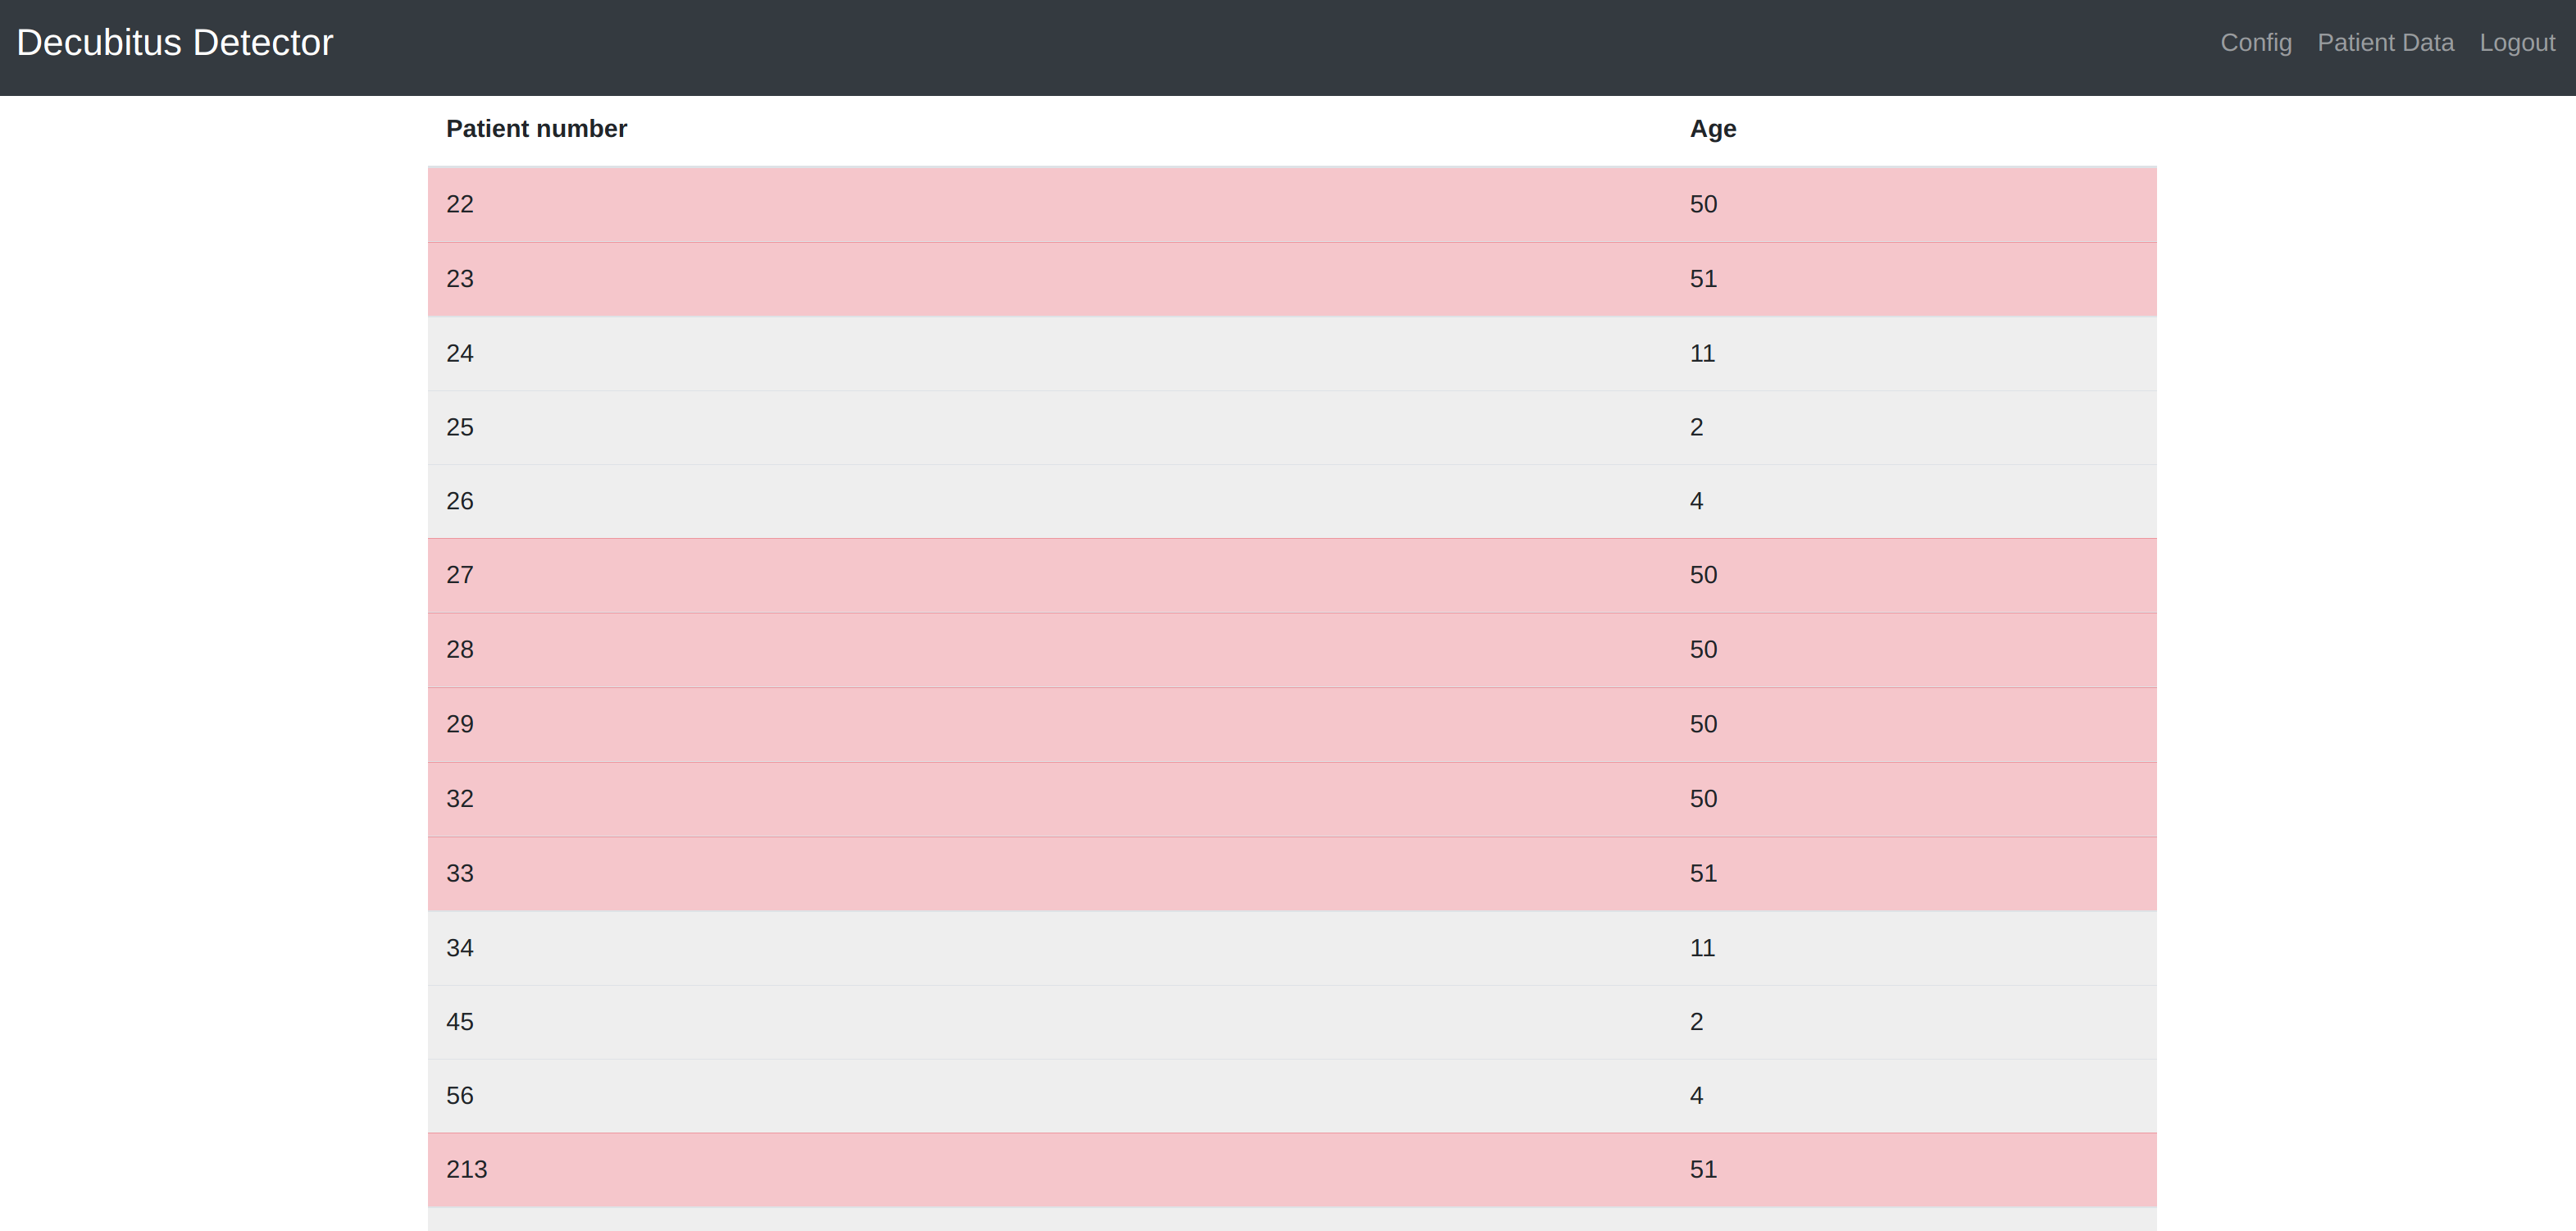
\includegraphics[width=0.45\linewidth]{images/gray.png}}
	& \num\putindeepbox[7pt]{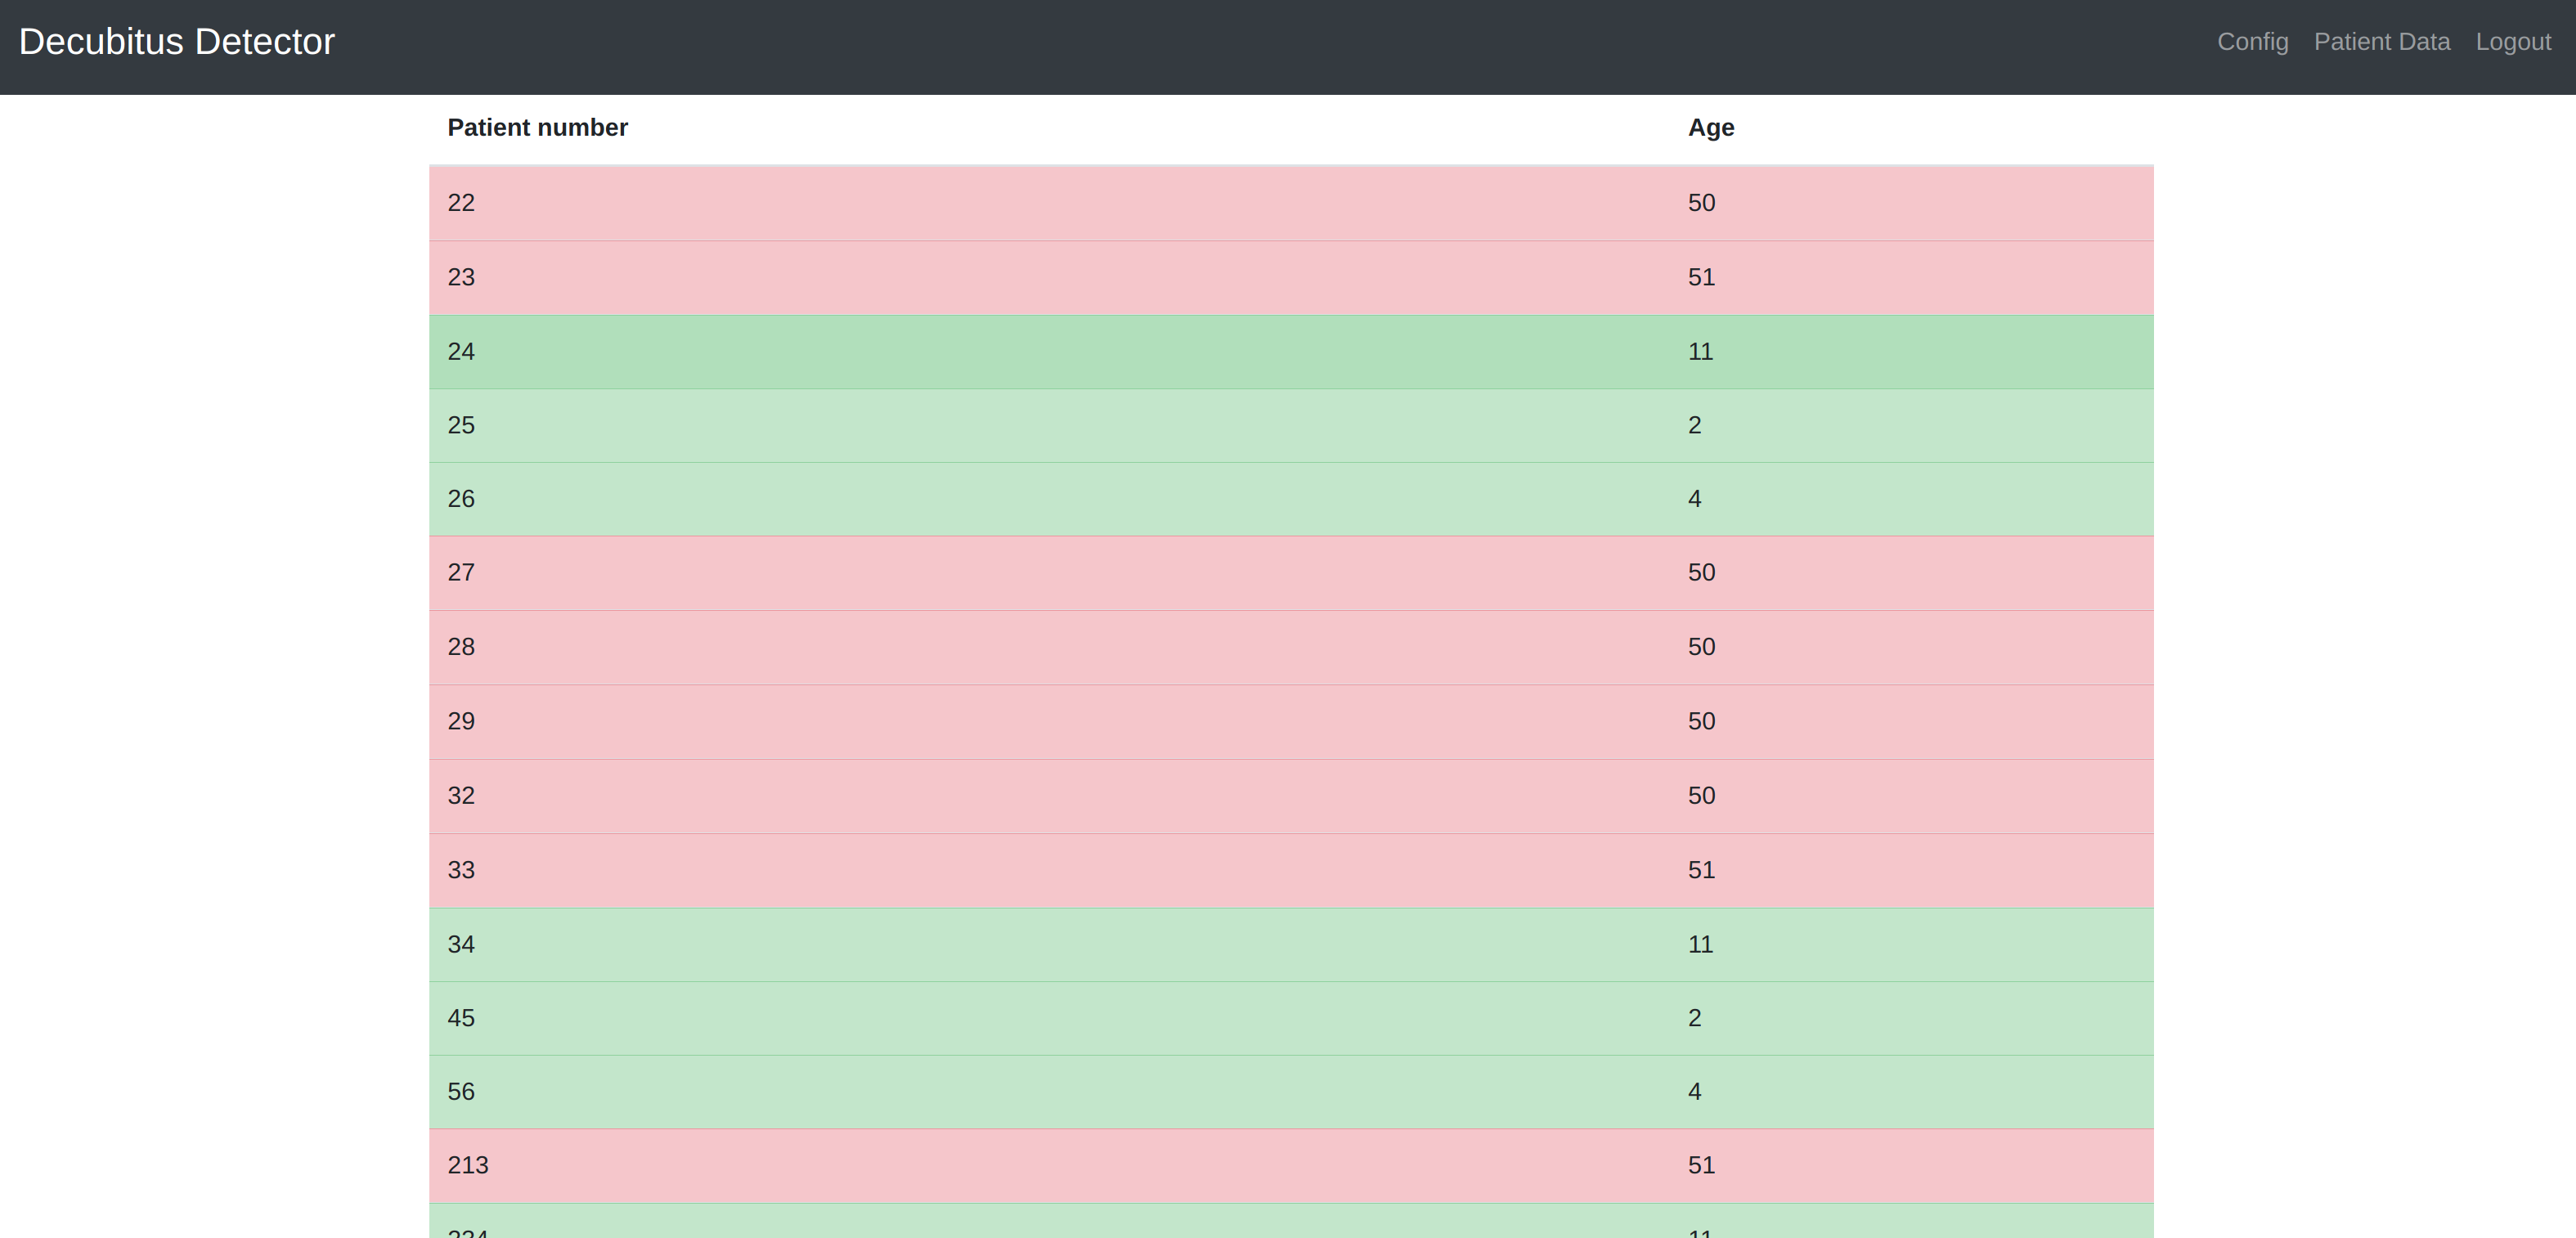
\includegraphics[width=0.45\linewidth]{images/green.png}} \\
	\num\putindeepbox[7pt]{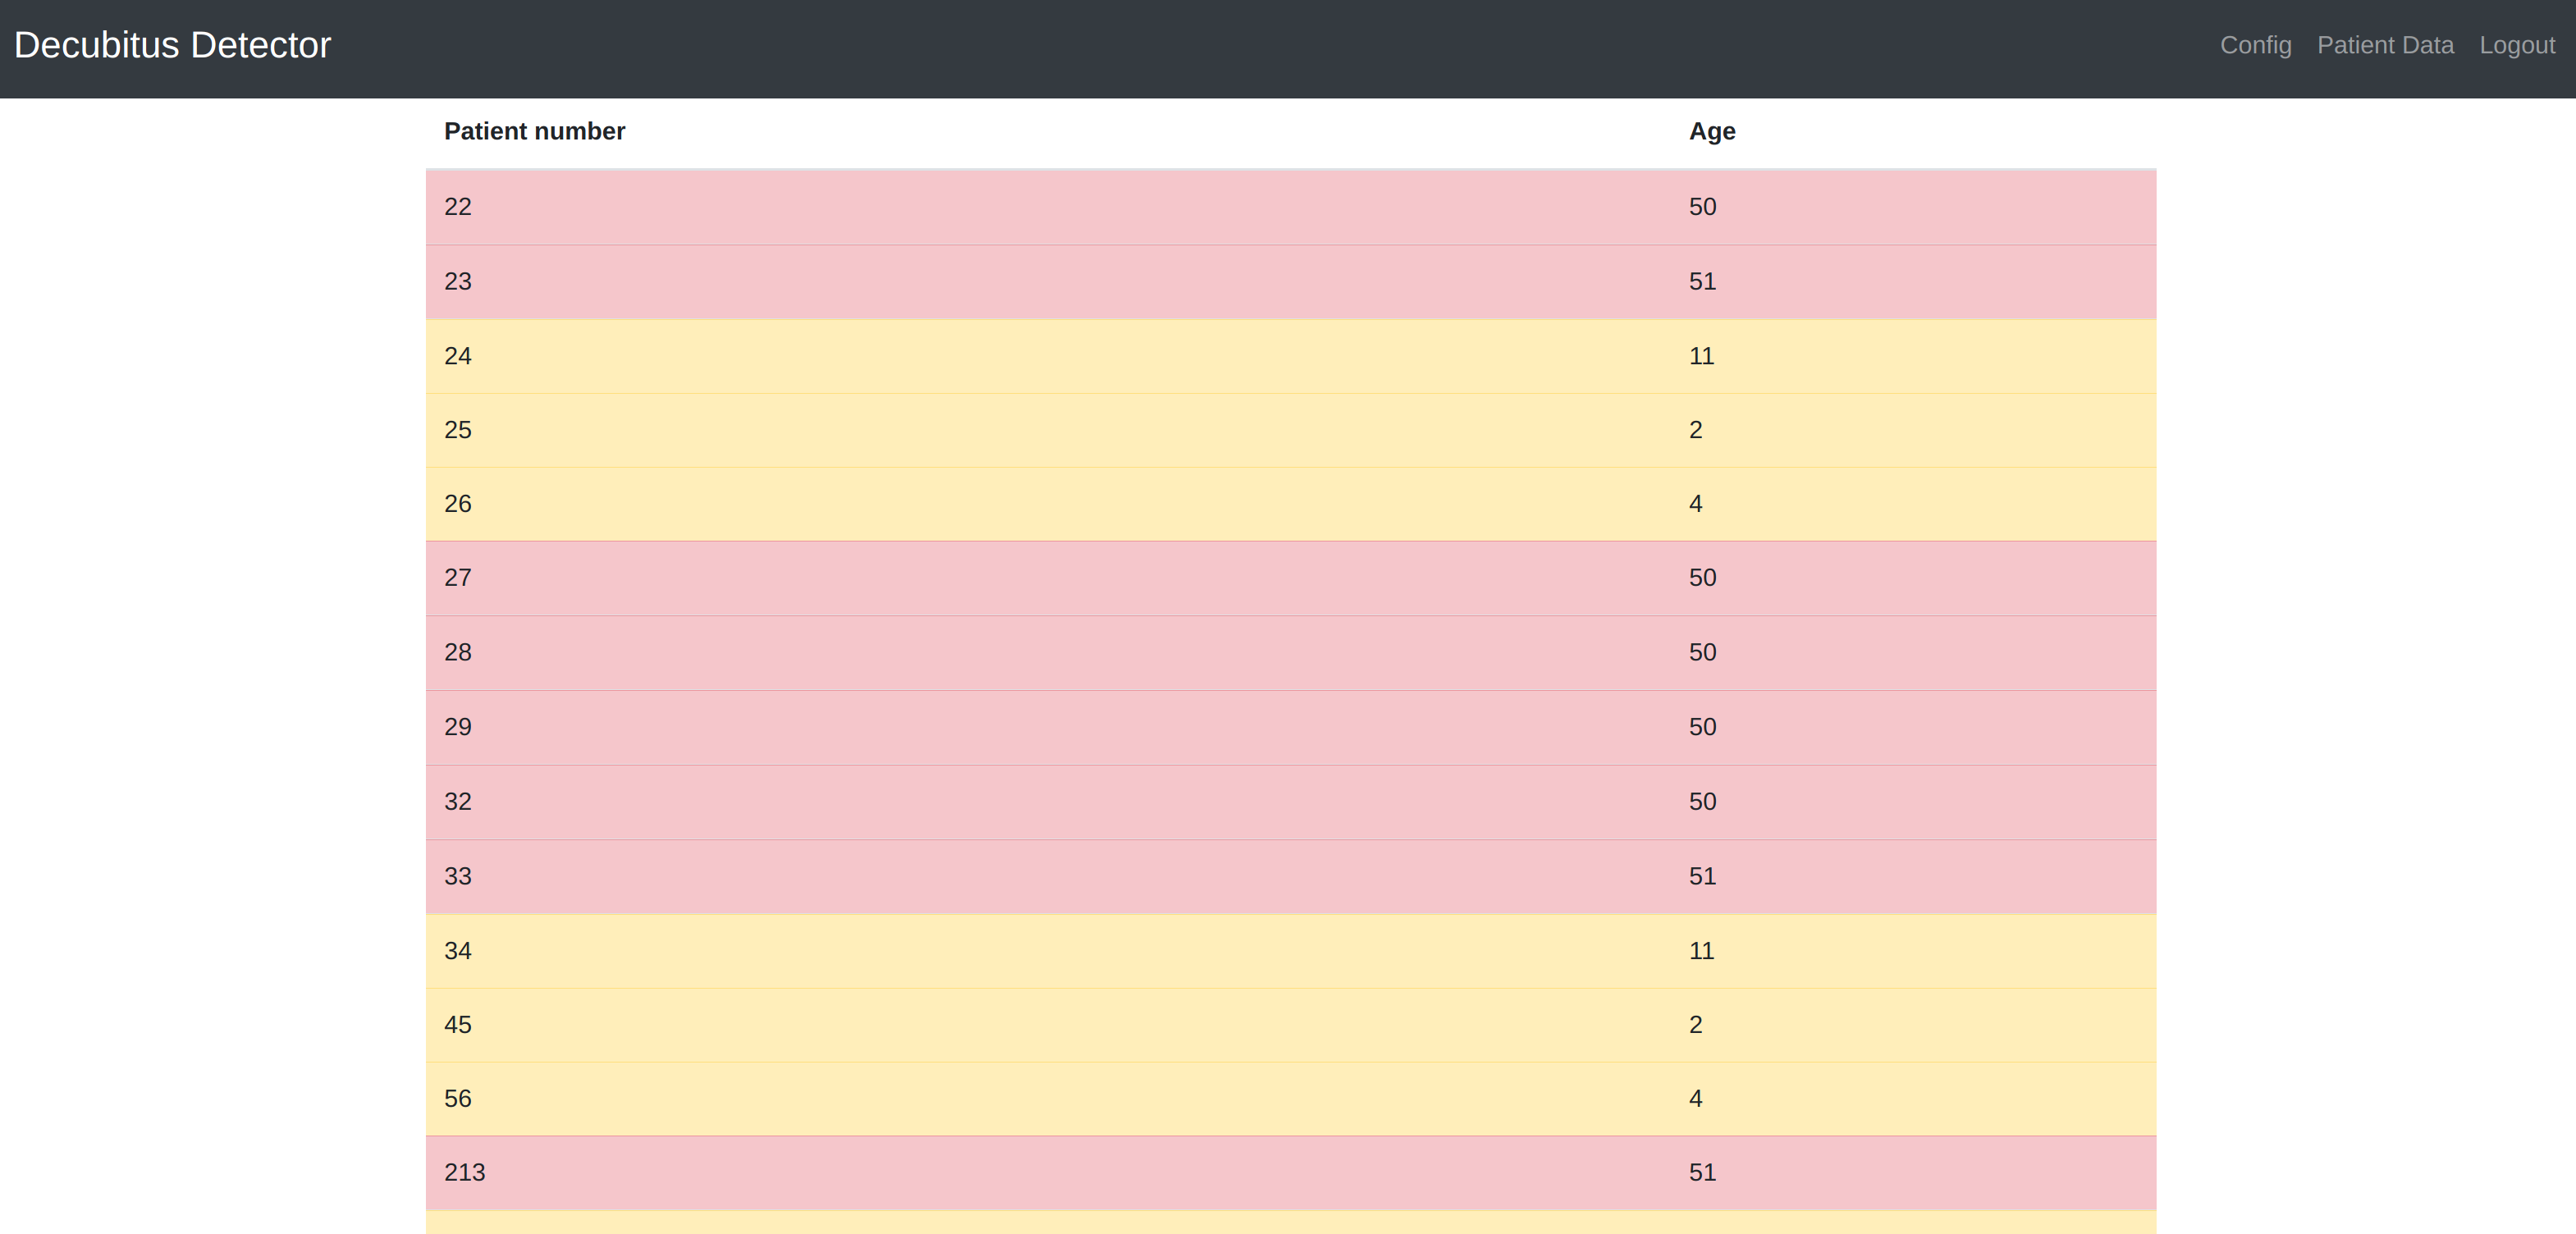
\includegraphics[width=0.45\linewidth]{images/yellow.png}}
	& \num\putindeepbox[7pt]{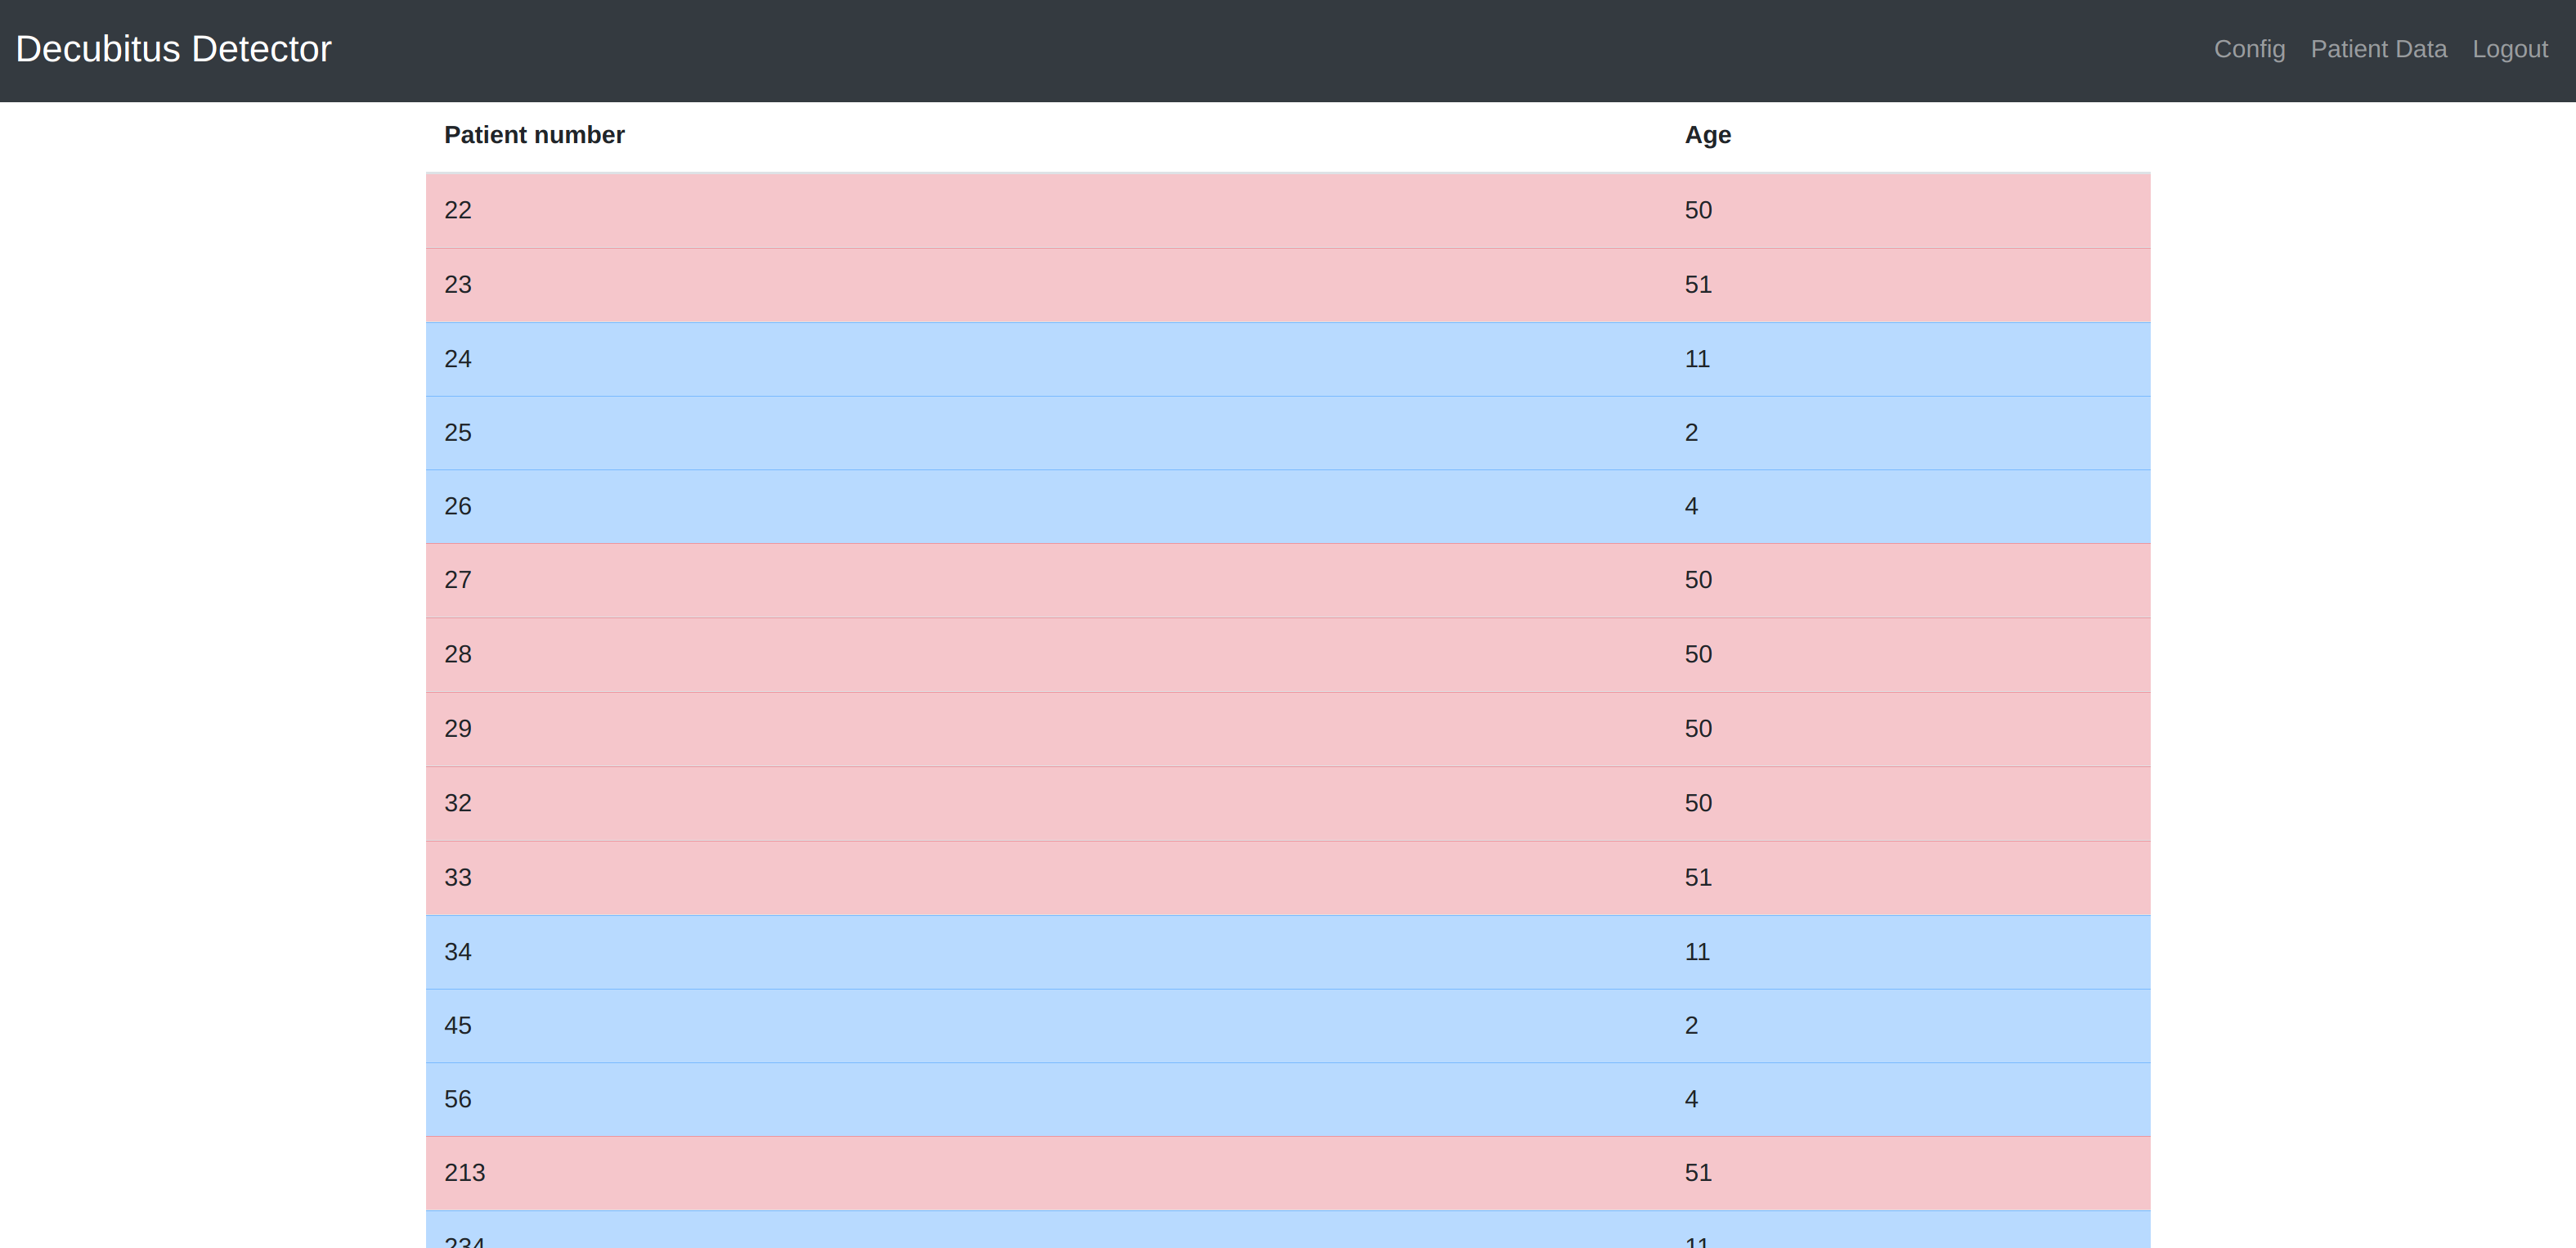
\includegraphics[width=0.45\linewidth]{images/blue.png}} \\
\end{tabular}


\iffalse
\begin{figure}[H]
	\centering
  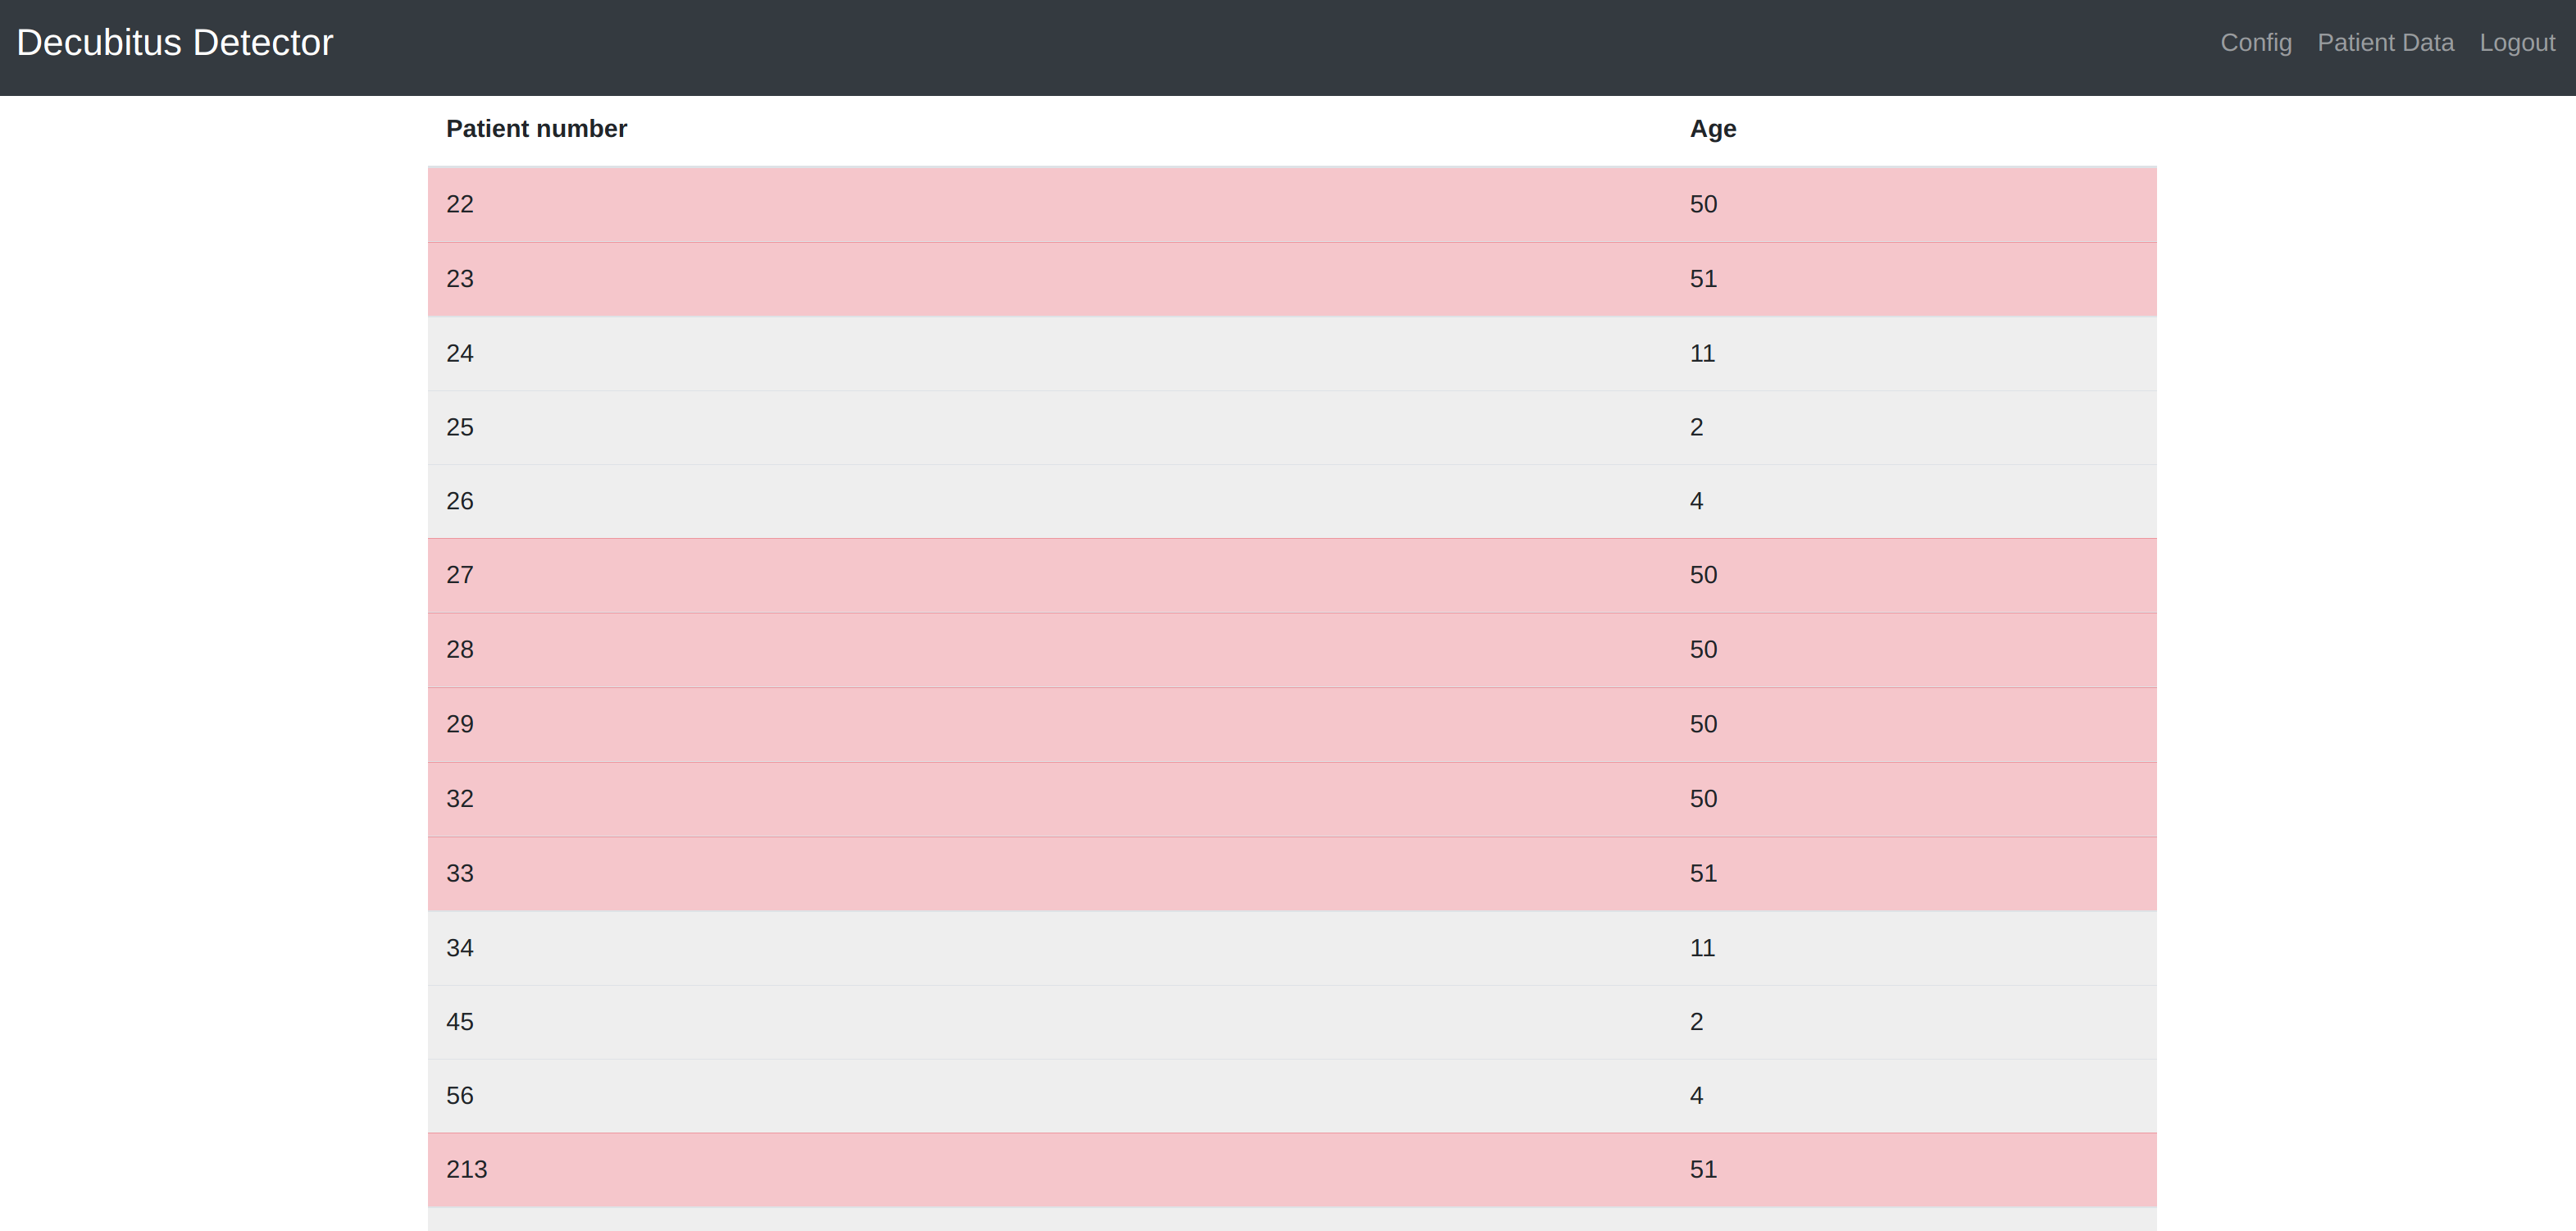
\includegraphics[width=0.8\linewidth]{images/gray.png}
	\captionsetup{labelformat=empty}
	\caption{a) Undetected patients are colorized in gray.}
  \label{fig:red}
\end{figure}

\begin{figure}[H]
	\centering
  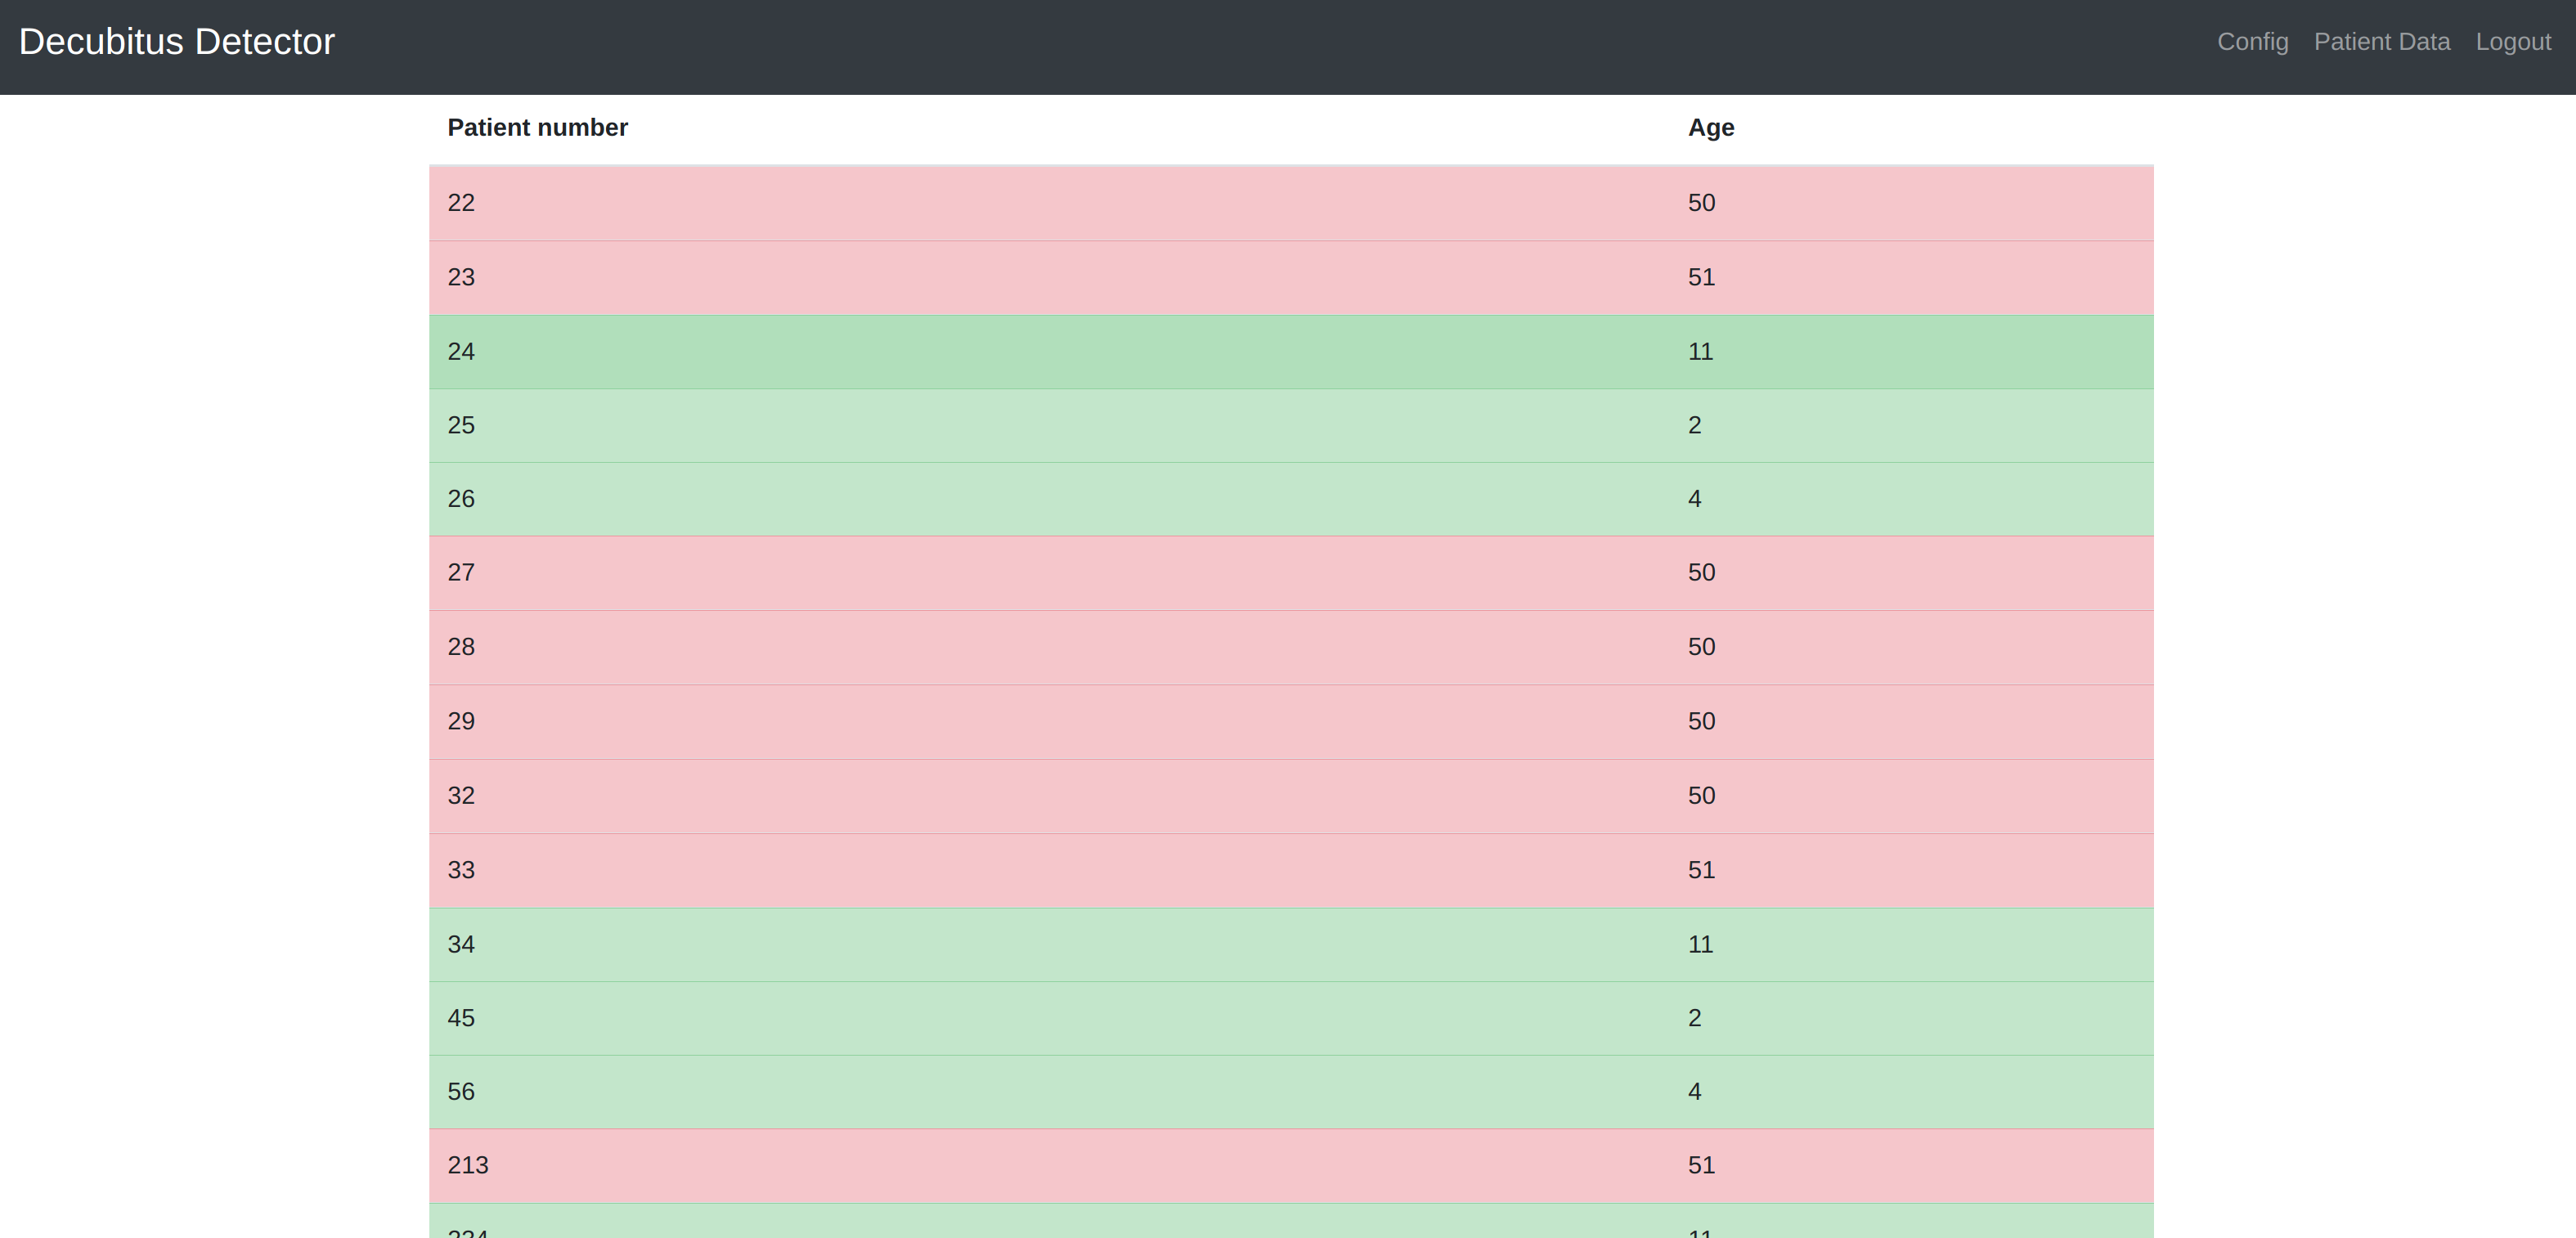
\includegraphics[width=0.8\linewidth]{images/green.png}
	\captionsetup{labelformat=empty}
	\caption{ b) Undetected patients are colorized in green.}
  \label{fig:green}
\end{figure}

\begin{figure}[H]
	\centering
  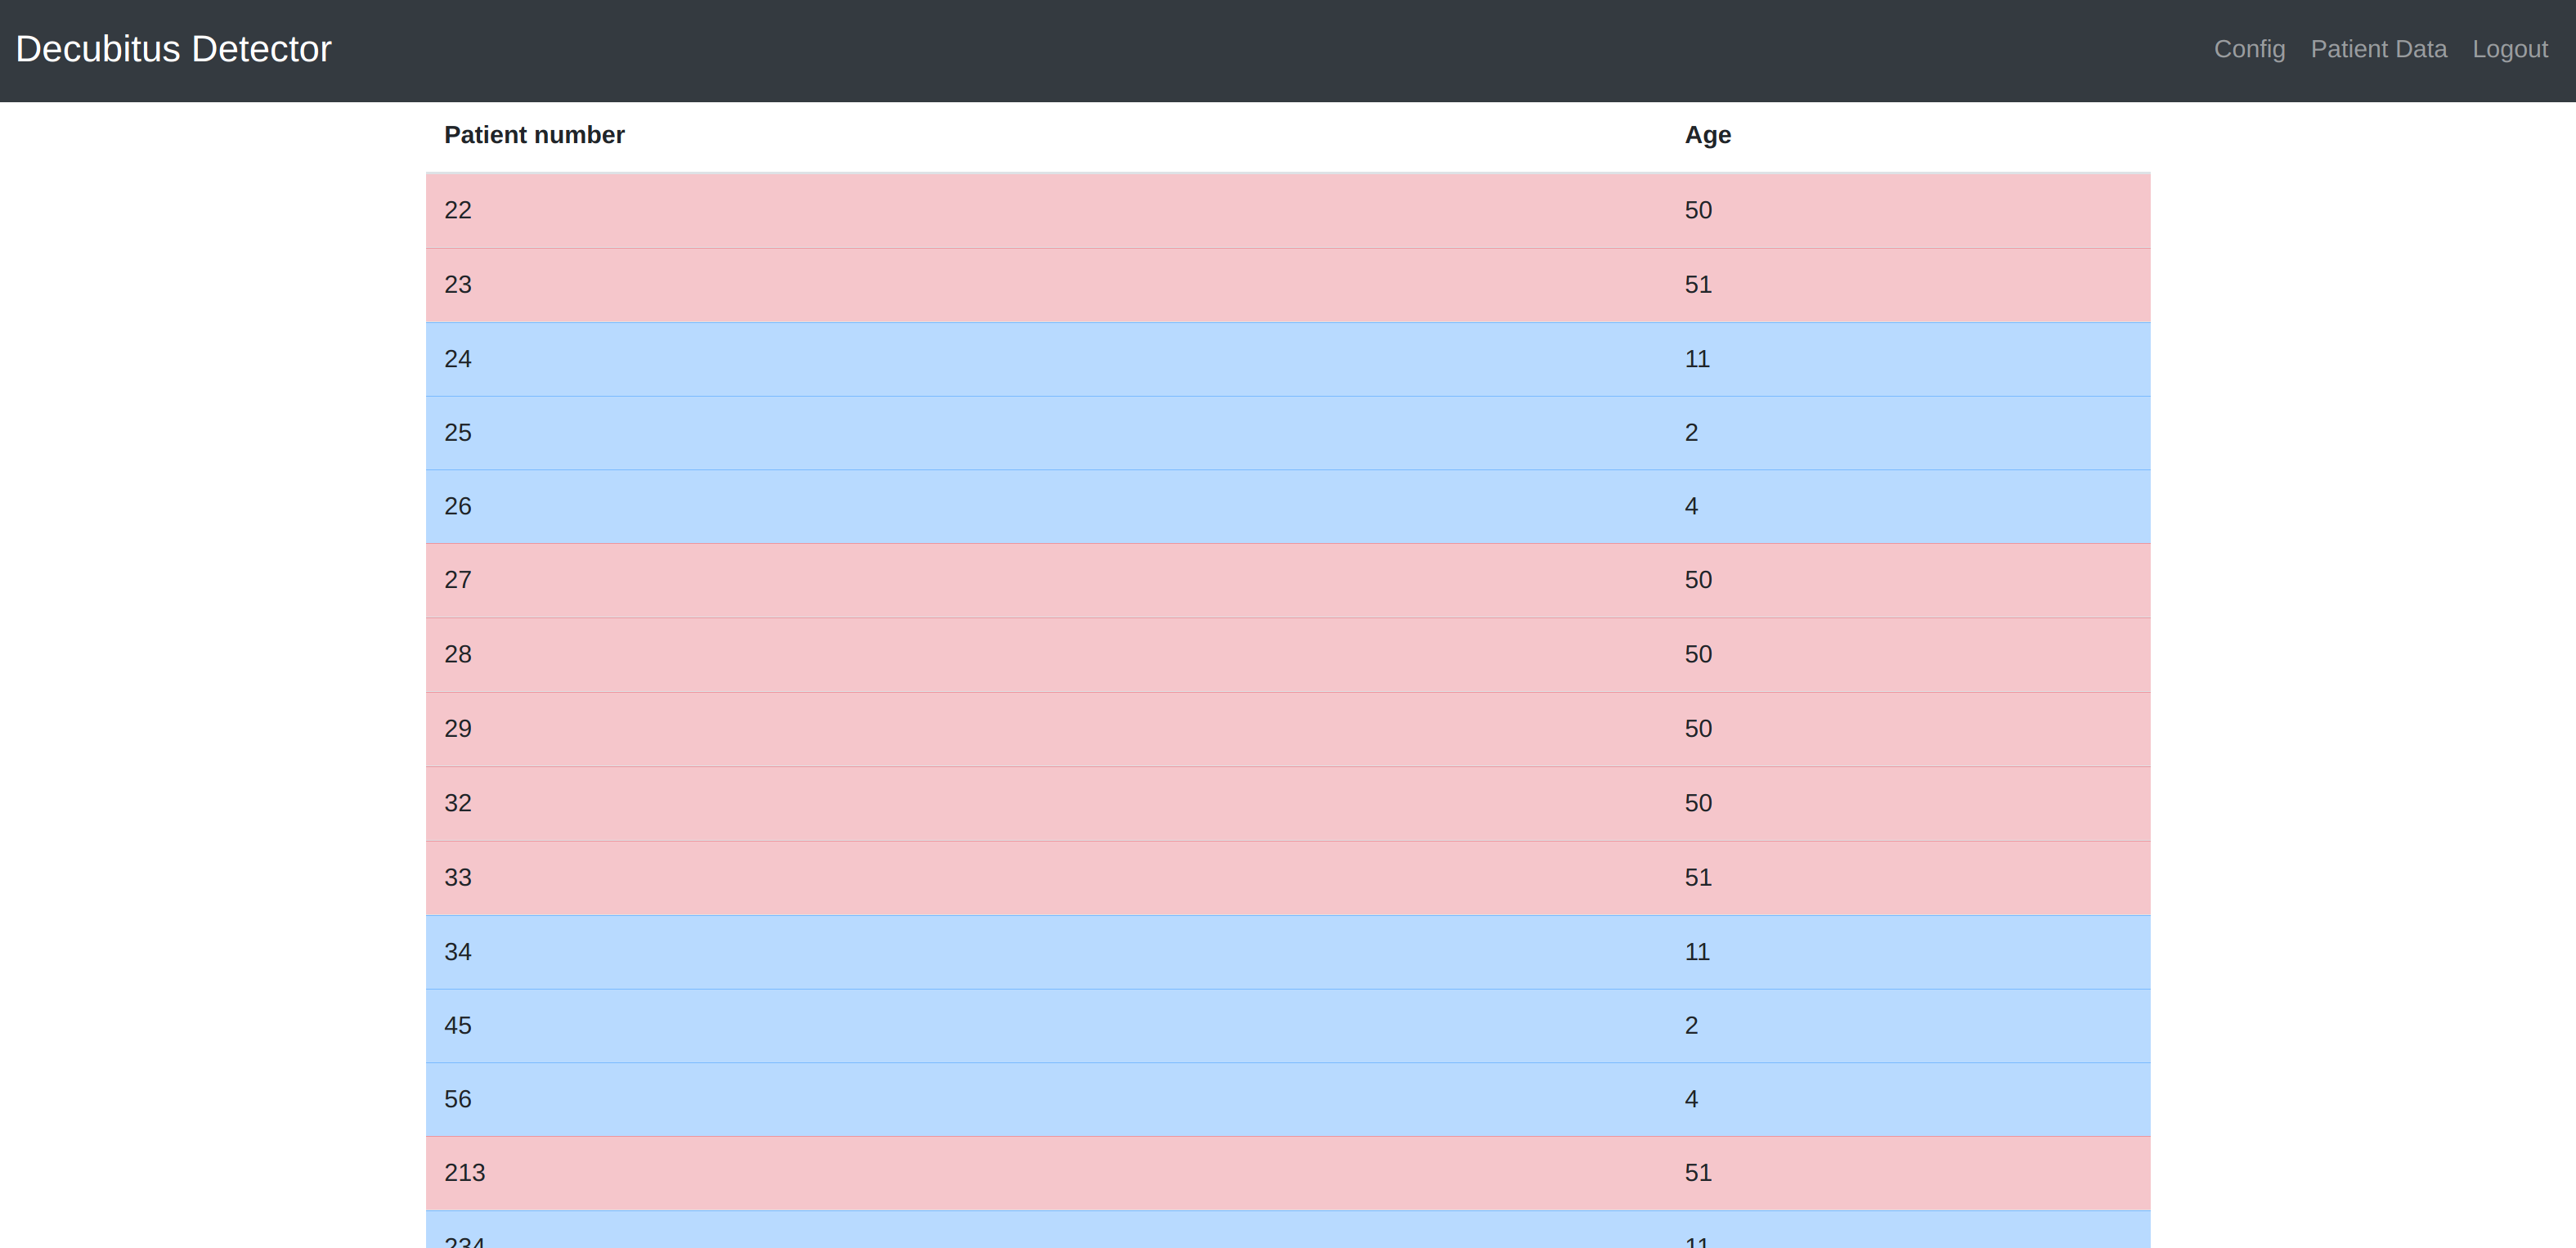
\includegraphics[width=0.8\linewidth]{images/blue.png}
	\captionsetup{labelformat=empty}
	\caption{c) Undetected patients are colorized in blue.}
  \label{fig:blue}
\end{figure}
\fi

\begin{questions}

\question Which color theme do you believe is the most suitable one?

\begin{checkboxes}
	\choice a) gray
	\choice b) green
	\choice c) yellow
	\choice d) blue
\end{checkboxes}

\end{questions}

\subsection*{Lists vs. Text}

\setcounter{eqn}{0}

The following images show the reasons, why our algorithm detected decubitus in different styles: As a list and as text. 

\begin{tabular}{cc}
	\num\putindeepbox[7pt]{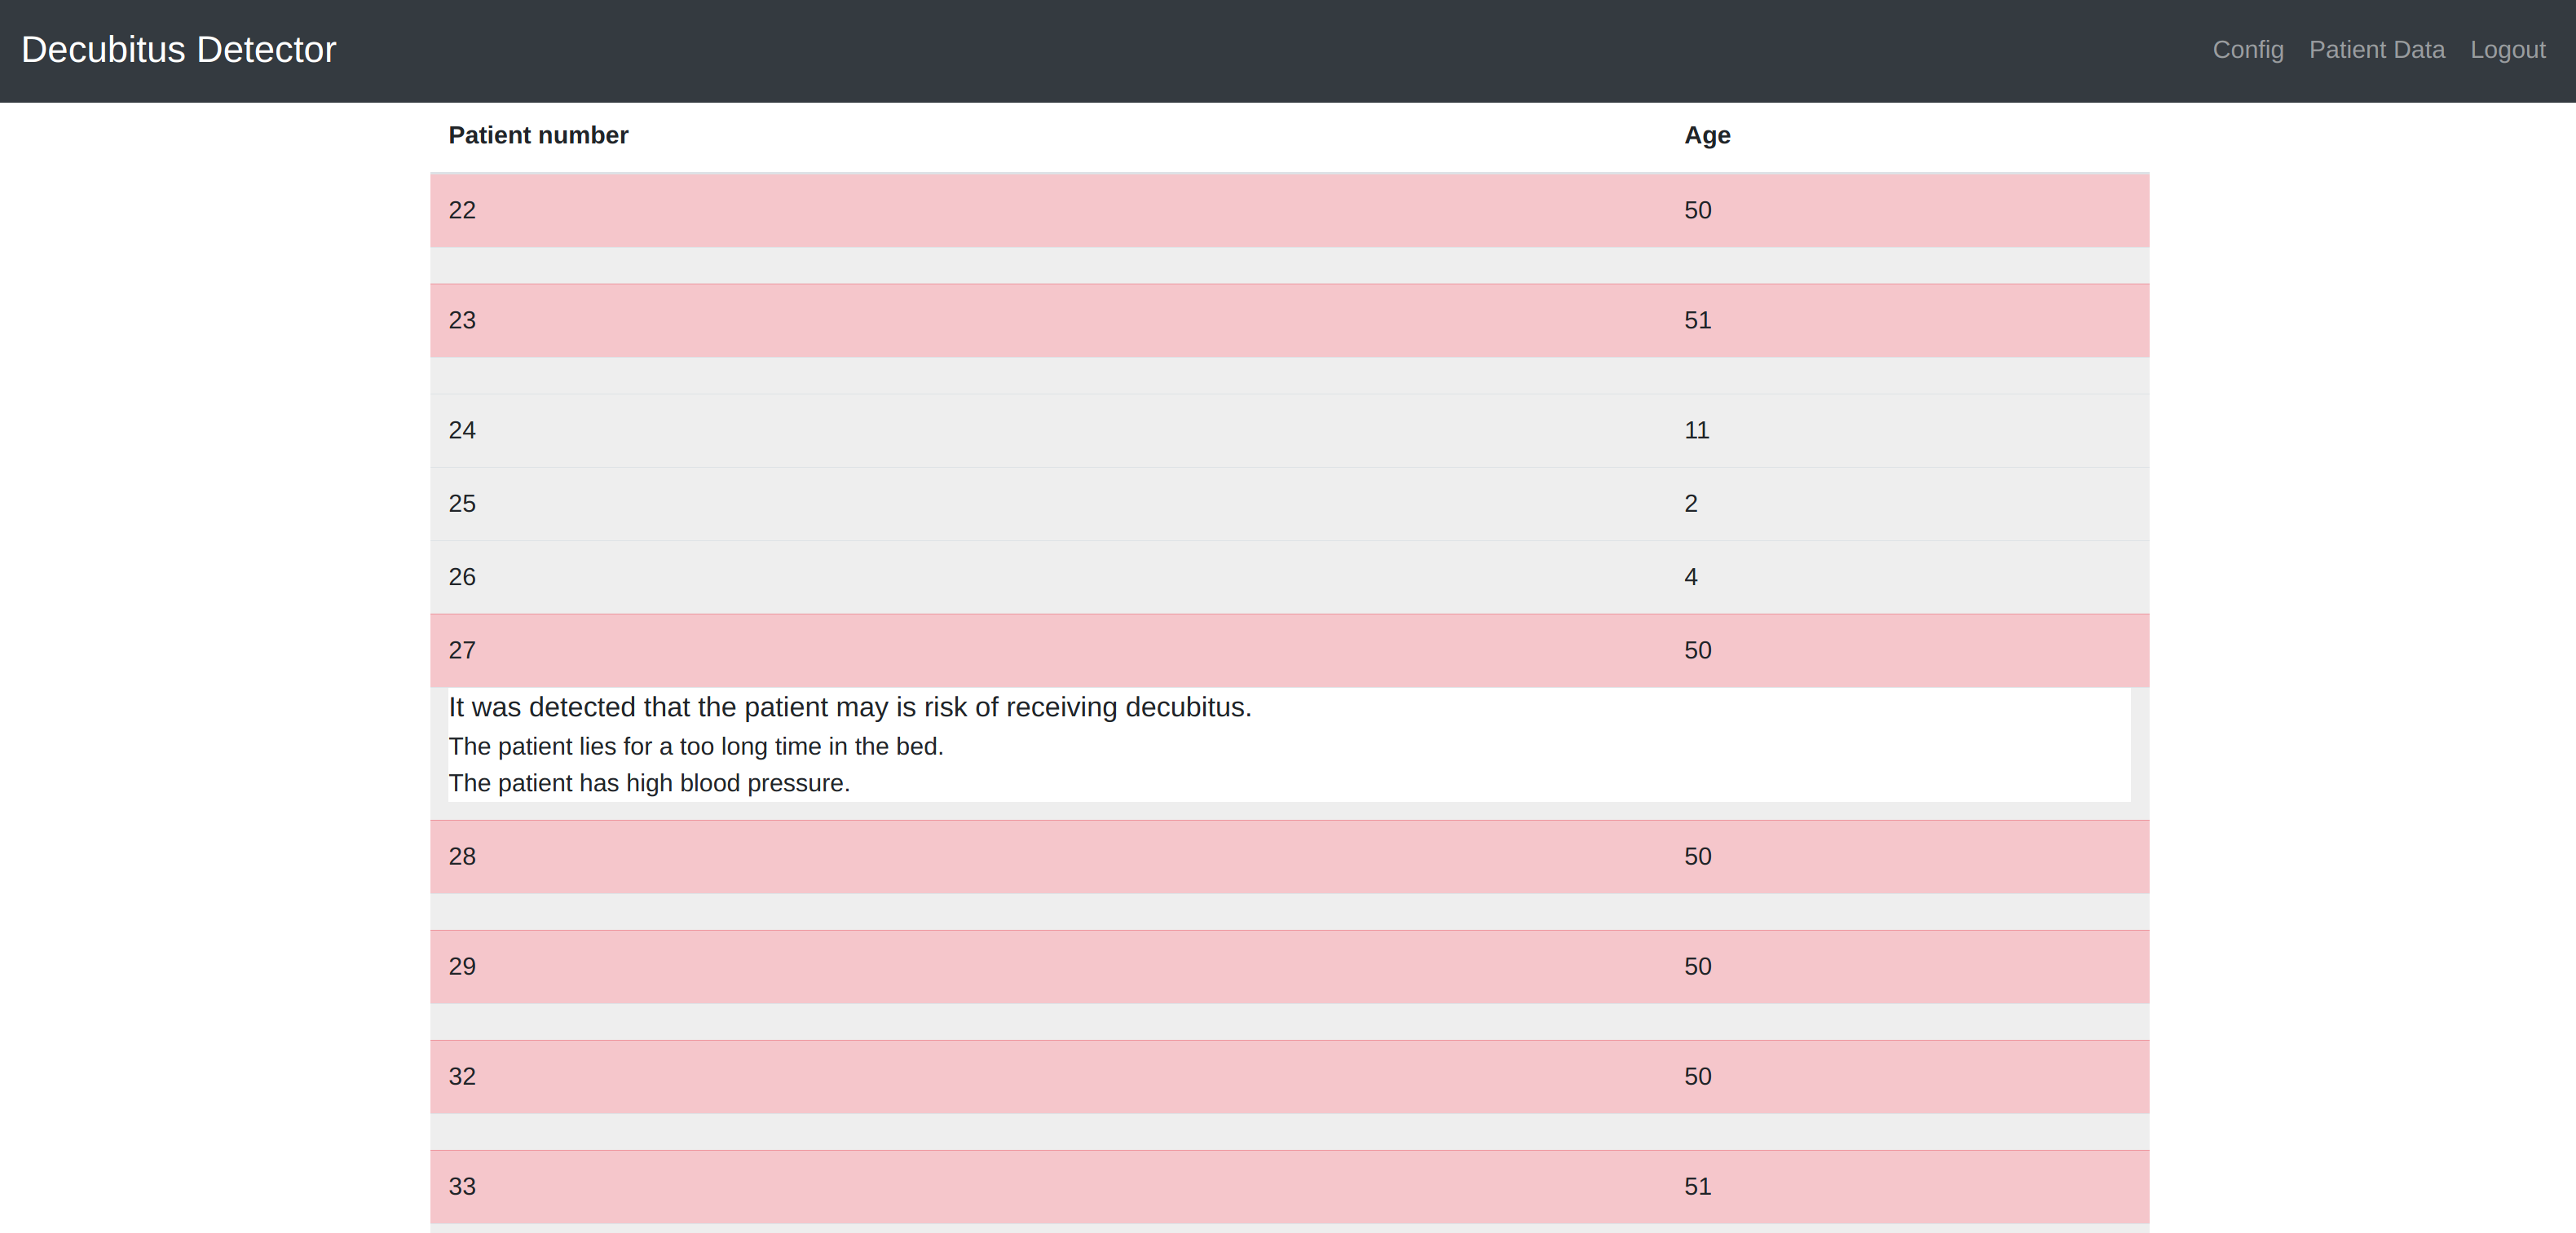
\includegraphics[width=0.45\linewidth]{images/text.png}}
	& \num\putindeepbox[7pt]{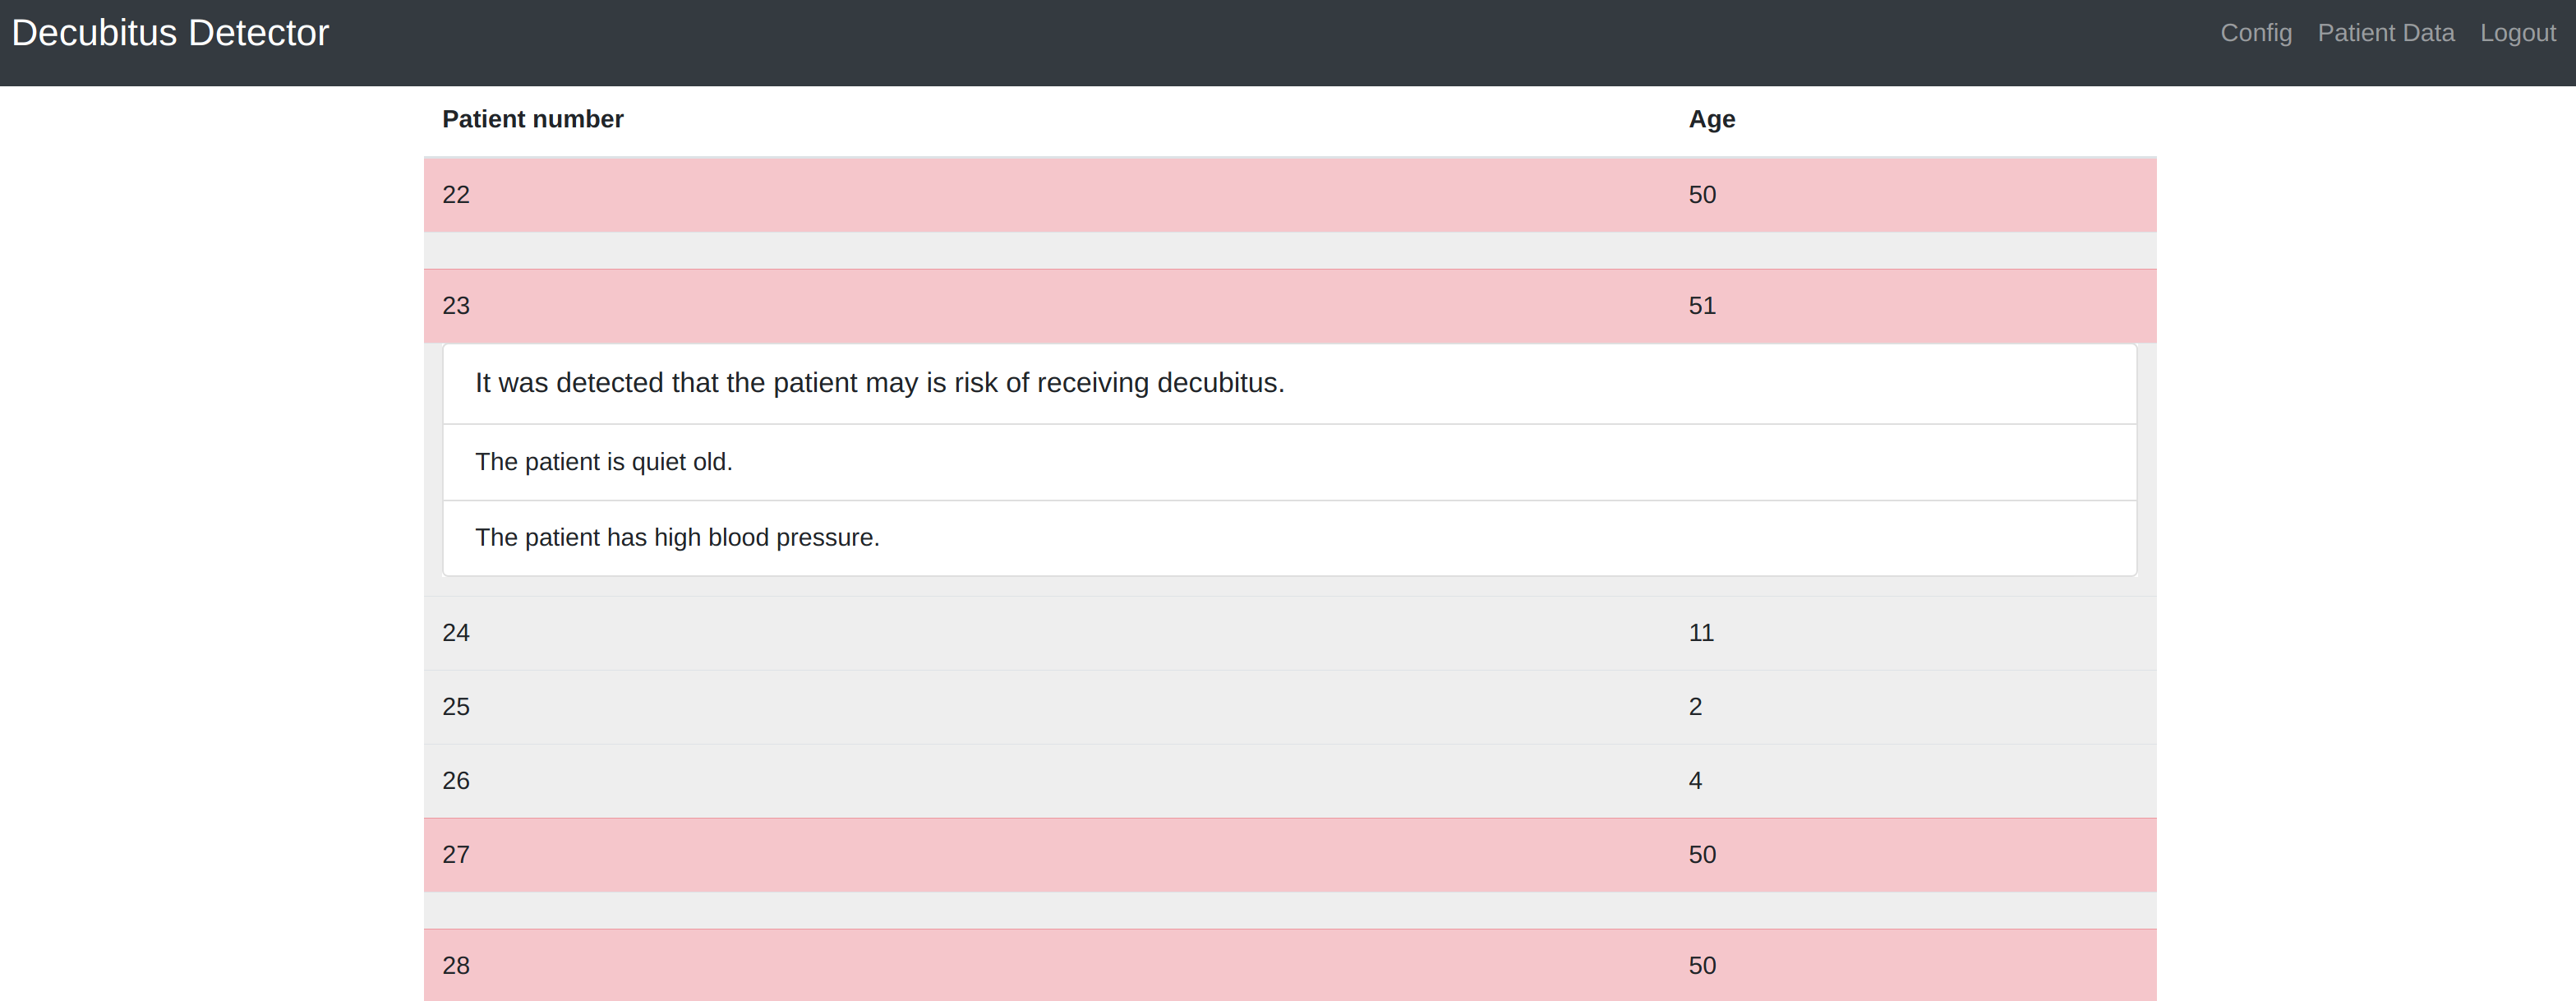
\includegraphics[width=0.45\linewidth]{images/lists.png}} \\
\end{tabular}

\iffalse
\begin{figure}[H]
	\centering
  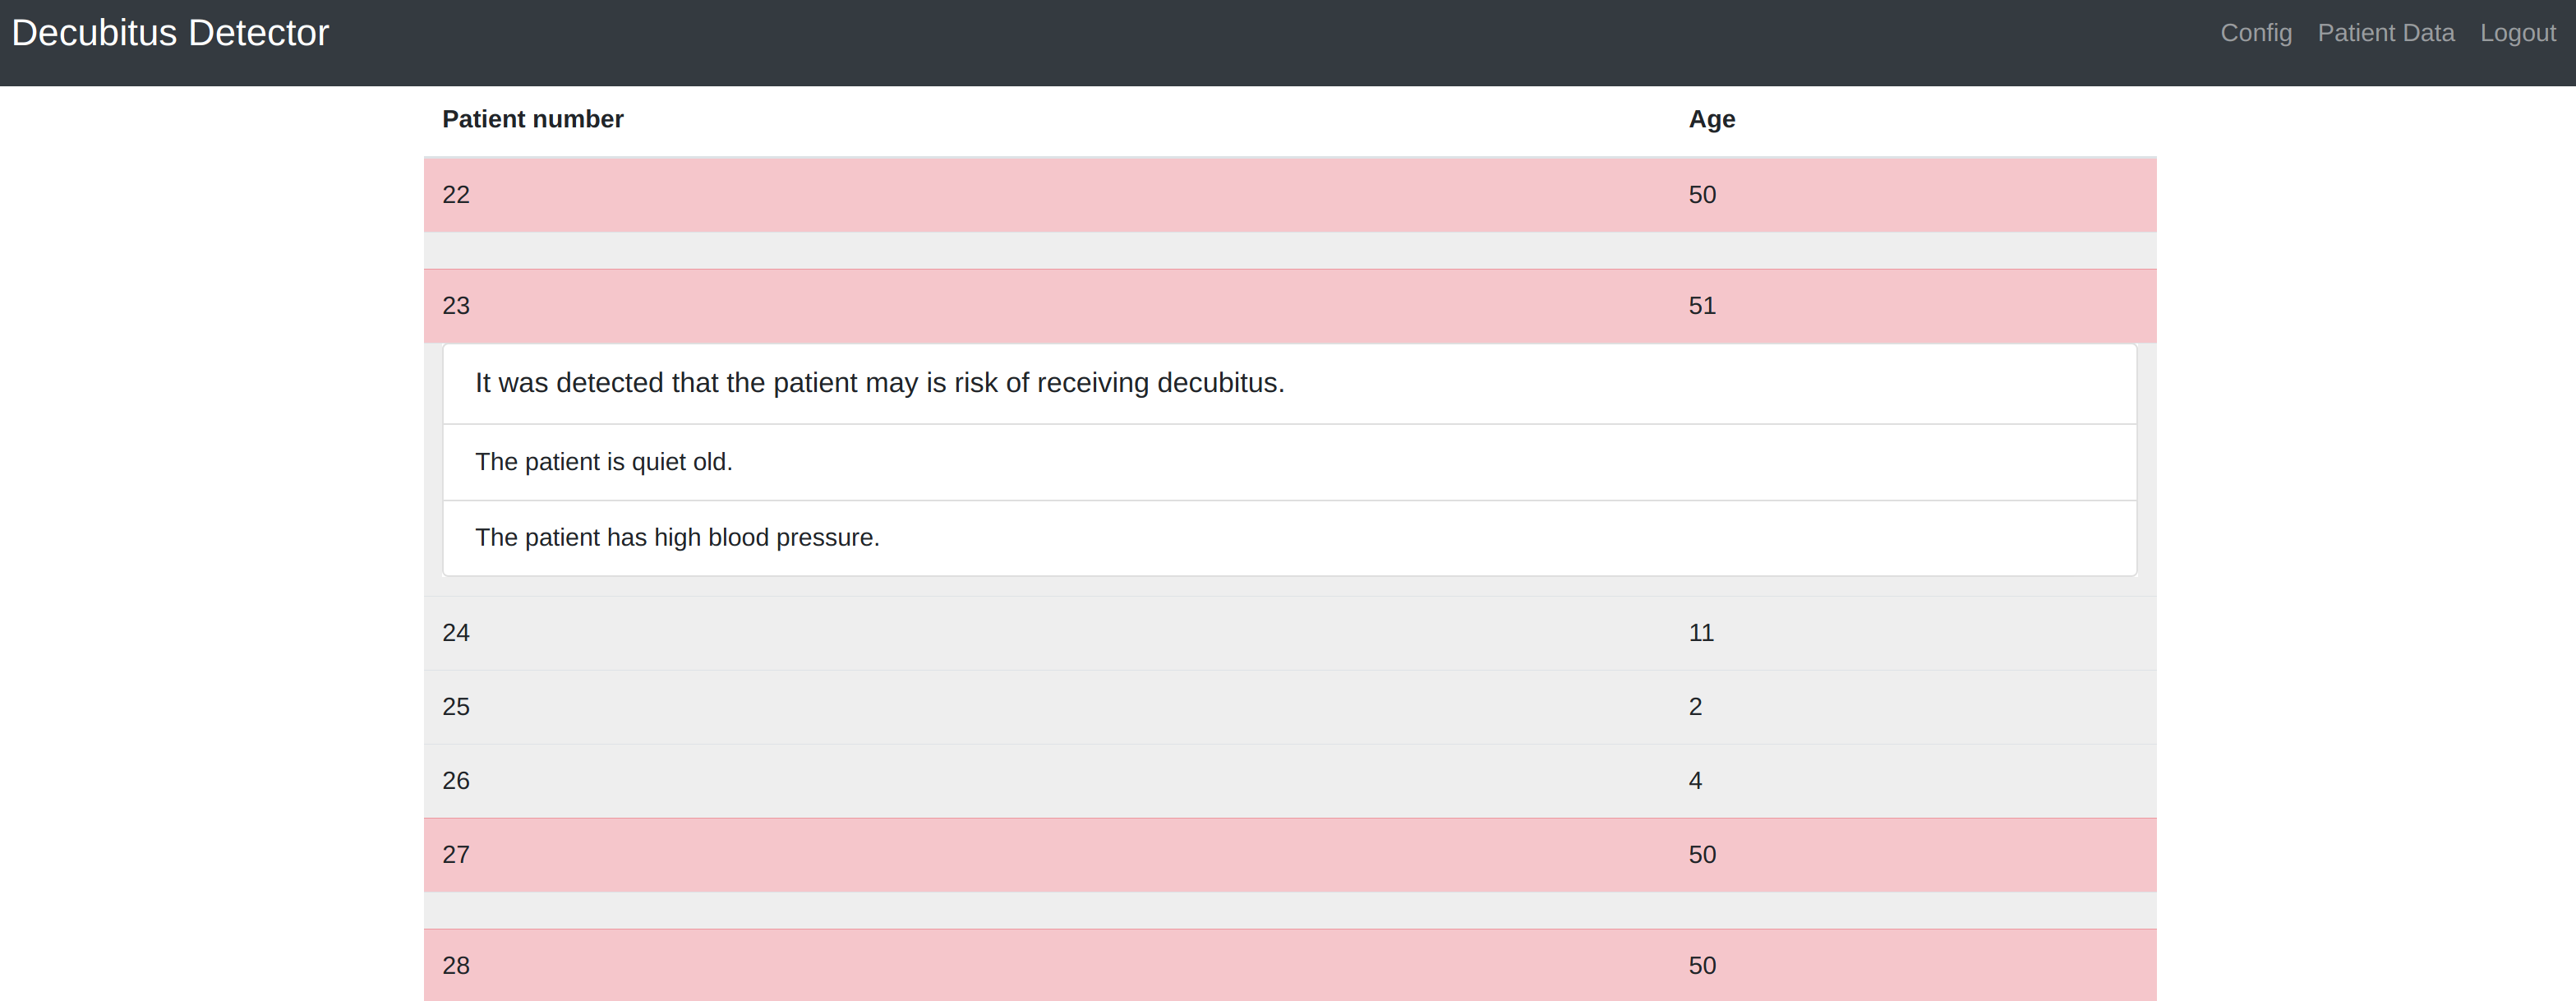
\includegraphics[width=0.8\linewidth]{images/lists.png}
	\captionsetup{labelformat=empty}
	\caption{ a) The explanation of the decision of our decision is illustrated as a list.}
  \label{fig:list}
\end{figure}

\begin{figure}[H]
	\centering
  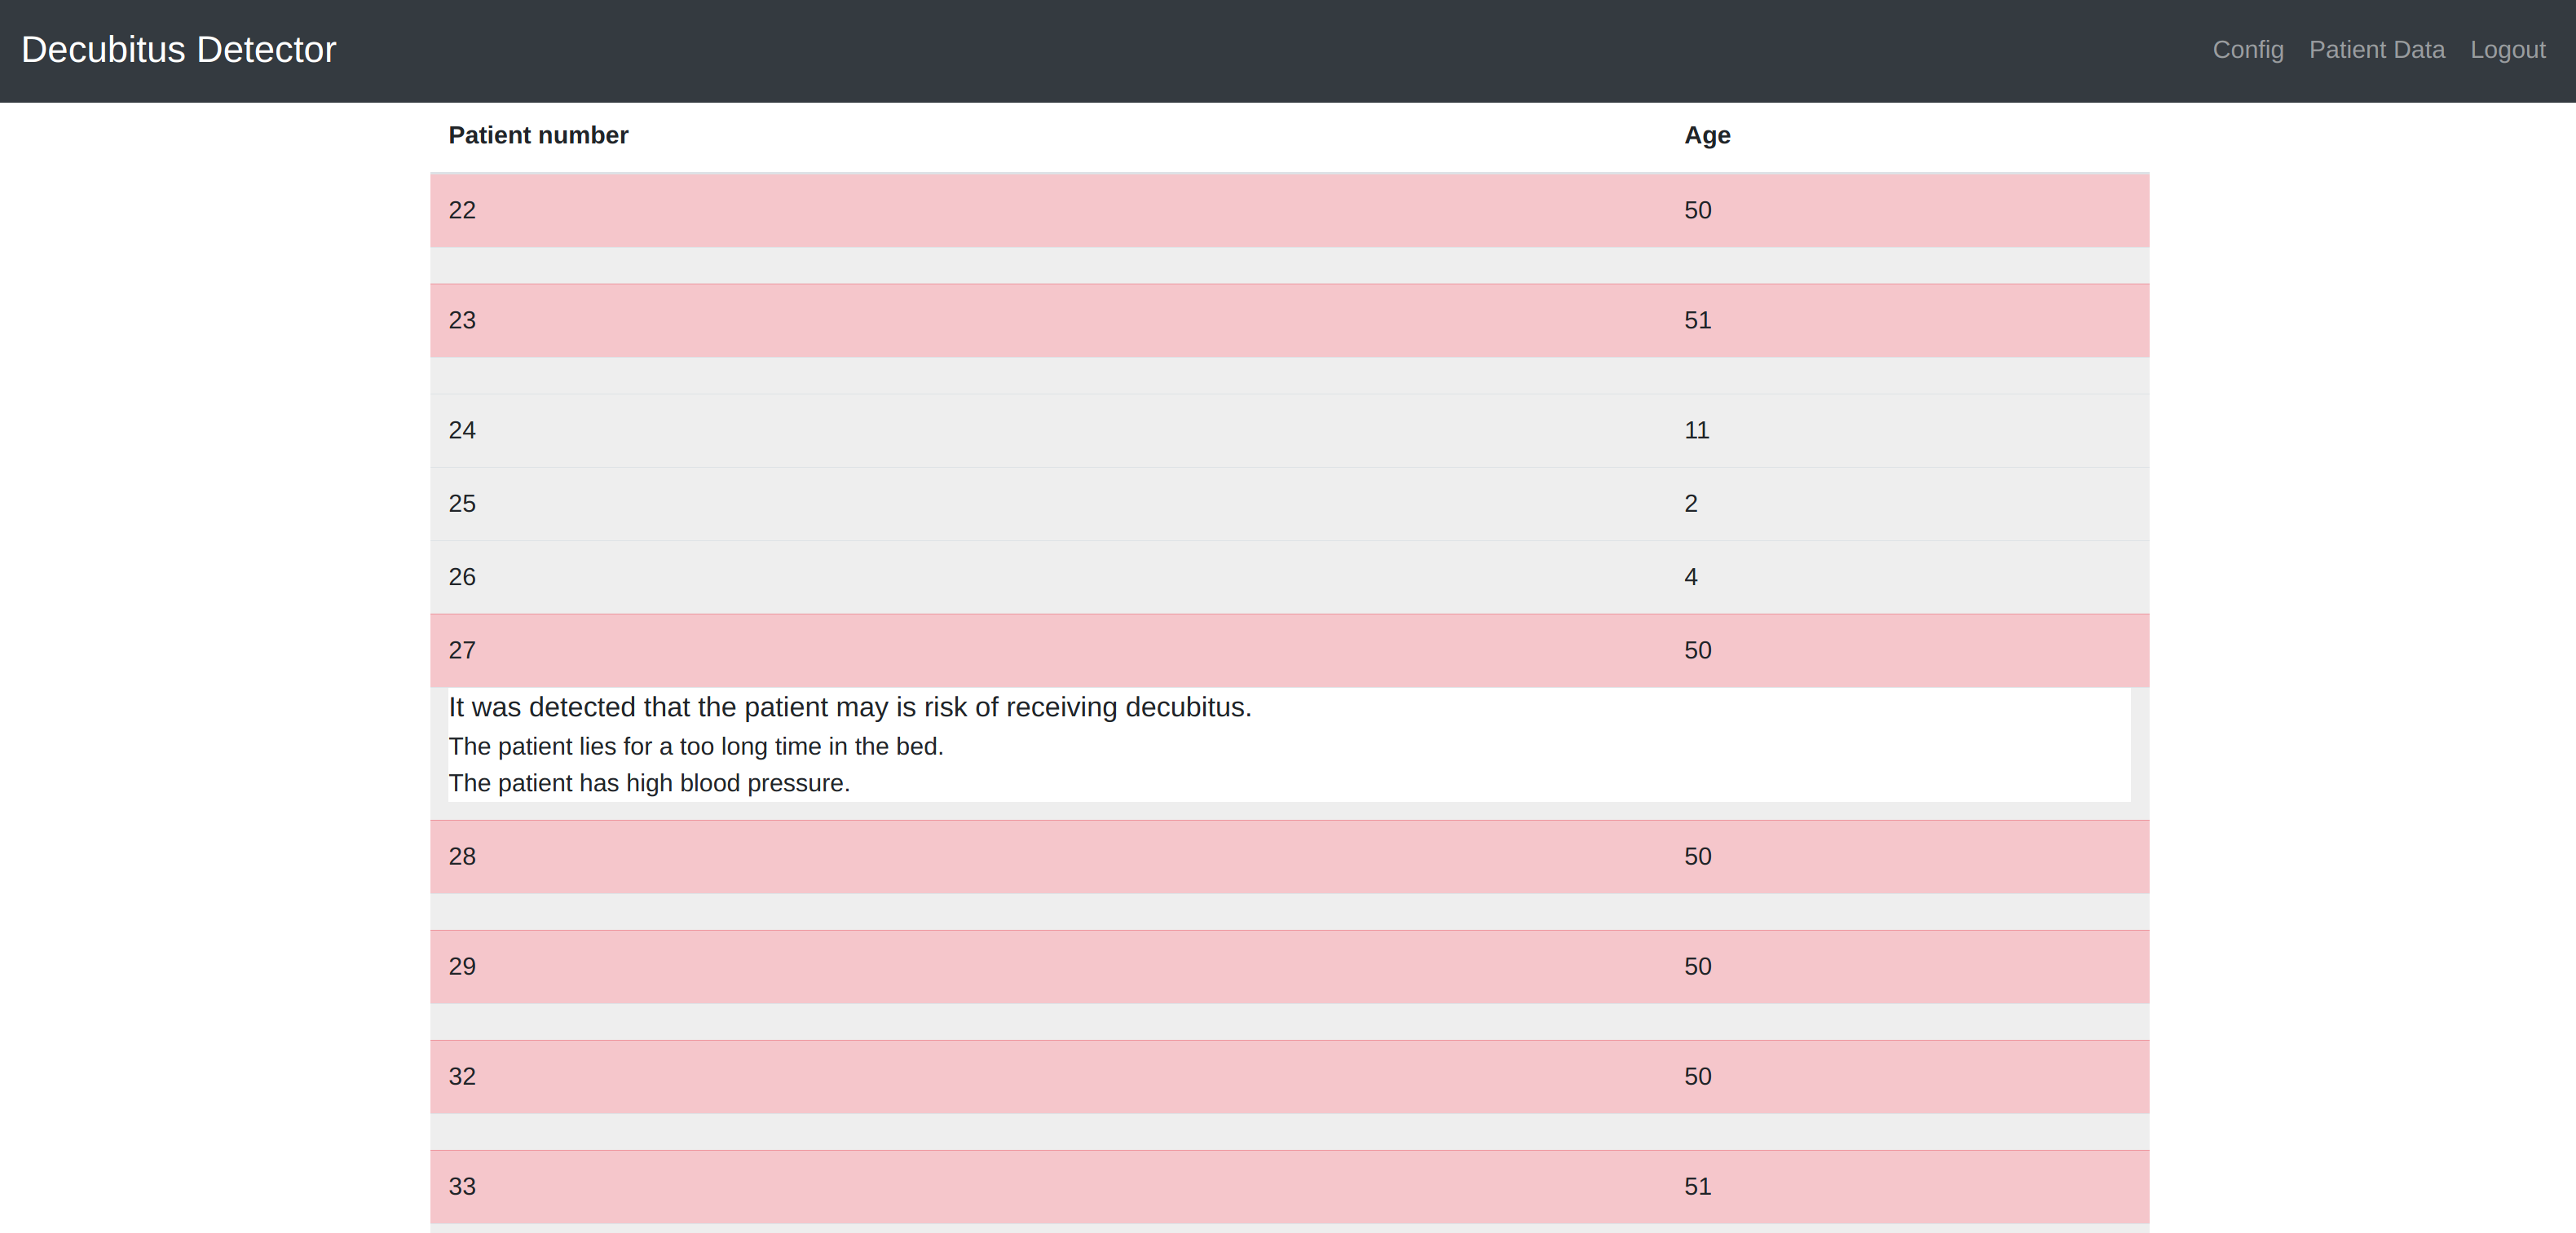
\includegraphics[width=0.8\linewidth]{images/text.png}
	\captionsetup{labelformat=empty}
	\caption{b) The explanation of the decision of the algorithm is illustrated as a text.}
  \label{fig:text}
\end{figure}
\fi

\begin{questions}

\question Would you prefer a text or a list?

\begin{checkboxes}
	\choice a) list
	\choice b) text
\end{checkboxes}

\end{questions}

\subsection*{Database Settings}

The frontend is completely separated from the ETL process and the detection algorithm. It just shows the results, stored in a database. 
But still, the database settings must be configured. Should database connection settings, such as hostname, port, username and password
be accessible from the frontend?\\
The following image shows how the configuration page may look like. \\
Note: As the frontend is basically a website, a server admin will still be able to modify the settings.

\begin{figure}[H]
	\centering
  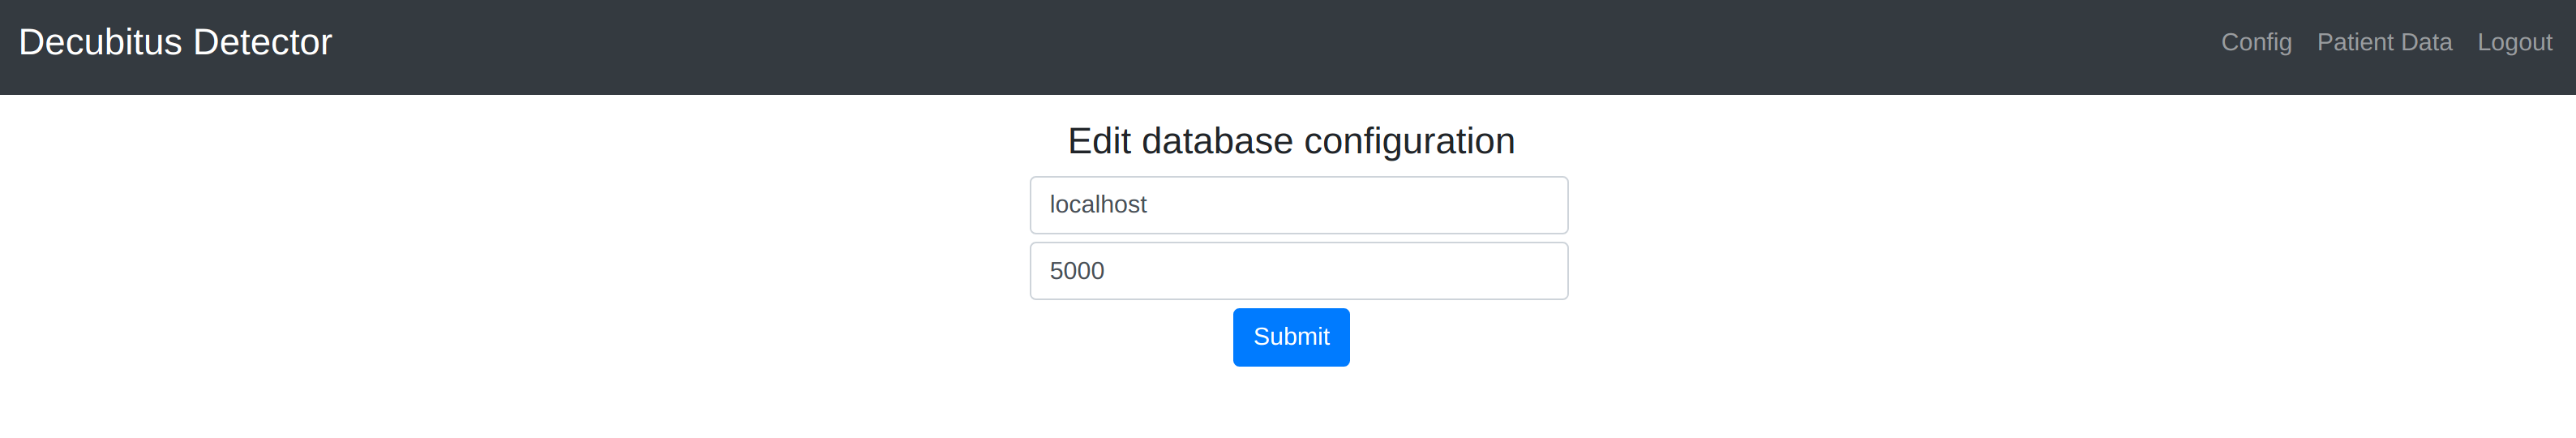
\includegraphics[width=0.8\linewidth]{images/db.png}
	\captionsetup{labelformat=empty}
	\caption{The config page.}
  \label{fig:text}
\end{figure}

\begin{questions}
\question Would you give the doctor the option to modify the database settings?

\begin{checkboxes}
	\choice Yes
	\choice No
\end{checkboxes}

\end{questions}

\subsection*{Patient Content}

Apart from reasons, why a patient is endangered, a doctor requires additional information (e.g. the patient id). 

\begin{questions}
\question Is it sufficient to show to show the ID of the patient along with his birth date?

\begin{checkboxes}
	\choice Yes
	\choice No
	\choice Doesn't matter
\end{checkboxes}

If you checked: "No", which additional information would you show the user?
\vspace{4cm}

\question Should there be an option to export the results as PDF file/a printable version?

\begin{checkboxes}
	\choice Yes
	\choice No
\end{checkboxes}

\question Which filter/sort options for the patients would you include?

	\begin{checkboxes}
		\choice Sort by detection (all endangered patients are shifted up)
		\choice Filter by patient ID
	\end{checkboxes}

	If you suggest additional filters, write them down below.
	\vspace{3cm}

\end{questions}

\subsection*{Credentials}

Medical records are highly confidential. One can prevent leaking data by an authentication system. The following image shows a login page.

\begin{figure}[H]
	\centering
  
\includegraphics[width=0.8\linewidth]{images/login.png}
	\captionsetup{labelformat=empty}
	\caption{The login page.}
  \label{fig:text}
\end{figure}

\begin{questions}
	\question Should we include the login page?

	\begin{checkboxes}
		\choice Yes
		\choice No
	\end{checkboxes}

\end{questions}

\section*{Backend}

Obviously the cron job for ETL and decubitus detection needs to be configured, according to several parameters. 
We recommend a short python script, which configures and starts the cron job. 


\begin{questions}

	\question Are simple command line arguments sufficient as configuration? \\E.g.: python3 cron.py --db\_port=1234 --db\_host=localhost

	\begin{checkboxes}
		\choice	Yes
		\choice	No
	\end{checkboxes}

	If you answered: "No", how should we include settings?

	\vspace{3cm}

	\question Which parameters are necessary? Please check them.

	\begin{checkboxes}
		\choice cron interval
		\choice database username
		\choice database password
		\choice database host
		\choice database port
		\choice location of the CSV files
		\choice logfile
	\end{checkboxes}
\end{questions}

\end{document}
